\documentclass[12pt,a4paper]{report}
\usepackage[utf8]{inputenc}
\usepackage[italian]{babel}
\usepackage{amsmath}
\usepackage{amsfonts}
\usepackage{xcolor}
\usepackage{color}
\usepackage{hyperref}
\usepackage{graphicx}
\usepackage{multicol}
\usepackage{wrapfig}
\usepackage{colortbl}
\usepackage[left=1.5cm,right=1.5cm,top=1cm,bottom=1.5cm]{geometry}
\usepackage{titlesec}
\usepackage{tikz}
\usepackage{svg}
\usepackage[off]{svg-extract}
\svgsetup{clean=true}

\hypersetup{
    colorlinks=true,
    linkcolor=black,
}

\definecolor{giallo}{rgb}{0.91, 0.84, 0.42}
\definecolor{celeste}{rgb}{0.61, 0.87, 1.0}
\definecolor{verde}{rgb}{0.66, 0.89, 0.63}
\definecolor{rosso}{rgb}{1.0, 0.25, 0.25}
\definecolor{viola}{RGB}{188, 135, 192}

\titleformat{\chapter}[hang]{\normalfont\huge\bfseries}{\thechapter.}{16pt}{\huge\bfseries}

\tikzset { attribute/.style ={shape = circle,fill = black}}
\begin{document}
 
\begin{titlepage}
    \newcommand{\HRule}{\rule{\linewidth}{0.5mm}}
    \center
    %\textsc{\LARGE Università di Pisa}\\[1.5cm]
    
\includegraphics[scale=0.8]{logo_black}\\[1.5cm]
    
\includegraphics[scale=1.4]{cherubino_black}\\[1cm]
    \textsc{\Large Dipartimento di Ingegneria dell'Informazione}\\[0.5cm]
    \textsc{\large CdL Ingegneria Informatica}\\[0.3cm] \textsc{\large Anno accademico 2021/2022} \\ [0.5cm]
    \HRule \\[0.4cm]
    { \huge \bfseries Documentazione Tecnica di Progetto}\\[0.4cm]
    \HRule \\[1cm]
    \begin{minipage}{1 \textwidth}
    \begin{center} \LARGE
        \emph{ \href{https://github.com/LombardiMatteo}{\textcolor{blue}{Matteo Lombardi}} $\quad$  \href{https://www.linkedin.com/in/francesco-zollo/}{\textcolor{blue}{Francesco Zollo}}}\\
    \end{center}
\end{minipage}\\[2cm]
\vfill
\end{titlepage}

\tableofcontents

\chapter{Glossario dei Termini}
    Affinchè l'utente possa usufruire della base di dati al pieno delle sue potenzialità e senza fraintenderne i contenuti, di seguito un elenco di termini ricorrenti e rilevanti associati ognuno alla propria descrizione, che ne esplica il significato interpretato ai fini del database.

    \begin{center}
        \begin{tabular}{|p{3cm}|p{8cm}|p{3cm}|}
            \hline
            \textbf{Termini} & \textbf{Descrizione} & \textbf{Sinonimi} \\
            \hline
            \rowcolor{giallo}
            \multicolumn{3}{|c|}{\textbf{Area Generale}} \\
            \hline
            % AREA GENERALE
            Edificio&Struttura costruita e/o ristrutturata che verrà in seguito monitorata.&Costruzione, Abitazione, Fabbricato, Stabile, Immobile \\
            \hline
            Pianta&Sezione orizzontale di un edificio all'altezza di un piano.&Mappa, Carta \\
            \hline
            Vano&Volume interno alla pianta delimitato da pareti, e adibito ad una o più funzioni. Di dimensione massime fisse.&Locale, Stanza \\
            \hline
            Punto d'Accesso&Punto che permette lo spostamento da un vano ad un altro oppure all'esterno. &Entrata, Uscita, Passaggio \\
            \hline
            Area Geografica&Porzione estesa di territorio terrestre delimitata da confini.&Stato, Paese \\
            \hline
            Rischio&Probabilità che un evento calamitoso, in una certa area geografica, sia capace di causare un certo danno agli edifici. & \\
            \hline
            % AREA COSTRUZIONE
            \rowcolor{celeste}
            \multicolumn{3}{|c|}{\textbf{Area Costruzione}} \\
            \hline
            Progetto&Insieme di lavori atti alla costruzione o alla ristrutturazione di un edificio.&Piano di lavoro \\
            \hline
            Lavoro&Attività svolte da operai con lo scopo di perseguire un progetto.& \\
            \hline
            Materiale&Mattone, intonaco, piastrella, pietra o altro, necessario a portare a termine un lavoro. & \\
            \hline
            Stadio&Stato di avanzamento in cui si trova un progetto.&Fase \\
            \hline
            Responsabile&Persona che monitora uno o più lavori.& \\
            \hline
            Turno&Data e orario (mattutino o pomeridiano) in cui un operaio o un capocantiere eseguirà un qualche lavoro. & \\
            \hline
            Lavoro Turno&Indicazione del lavoro svolto dall'operaio e/o dal capo cantiere, con relativo numero di ore, nel dato turno.& \\
            \hline
        \end{tabular}
            \newpage
               
        \begin{tabular}{|p{3cm}|p{8cm}|p{3cm}|}
            \hline
            \textbf{Termini} & \textbf{Descrizione} & \textbf{Sinonimi} \\
            % AREA MONITORAGGIO
            \hline
            \rowcolor{verde}
            \multicolumn{3}{|c|}{\textbf{Area Monitoraggio}} \\
            \hline
            Sensore&Dispositivo elettronico che misura un certo valore o un insieme di valori.&Dispositivo di controllo \\
            \hline
            Registrazione&Valore(i) misurato(i) da un certo sensore in un determinato momento.&Rilevazione \\
            \hline
            Alert&Avvertimento di pericolo, generato in seguito alla registrazione di un valore superiore ad una soglia, da un dato sensore in un certo tempo. & \\
            \hline
            \rowcolor{rosso}
             % AREA ANALISI DEL RISCHIO
            \multicolumn{3}{|c|}{\textbf{Area Analisi del Rischio}} \\
            \hline
            Calamità&Evento catastrofico di tipo sismico o idrogeologico verificatosi in una certa zona geografica in un certa data. & \\
            \hline
        \end{tabular}
    \end{center}


\part{Modello Concettuale}
\chapter{Area Generale}
    \begin{center}
        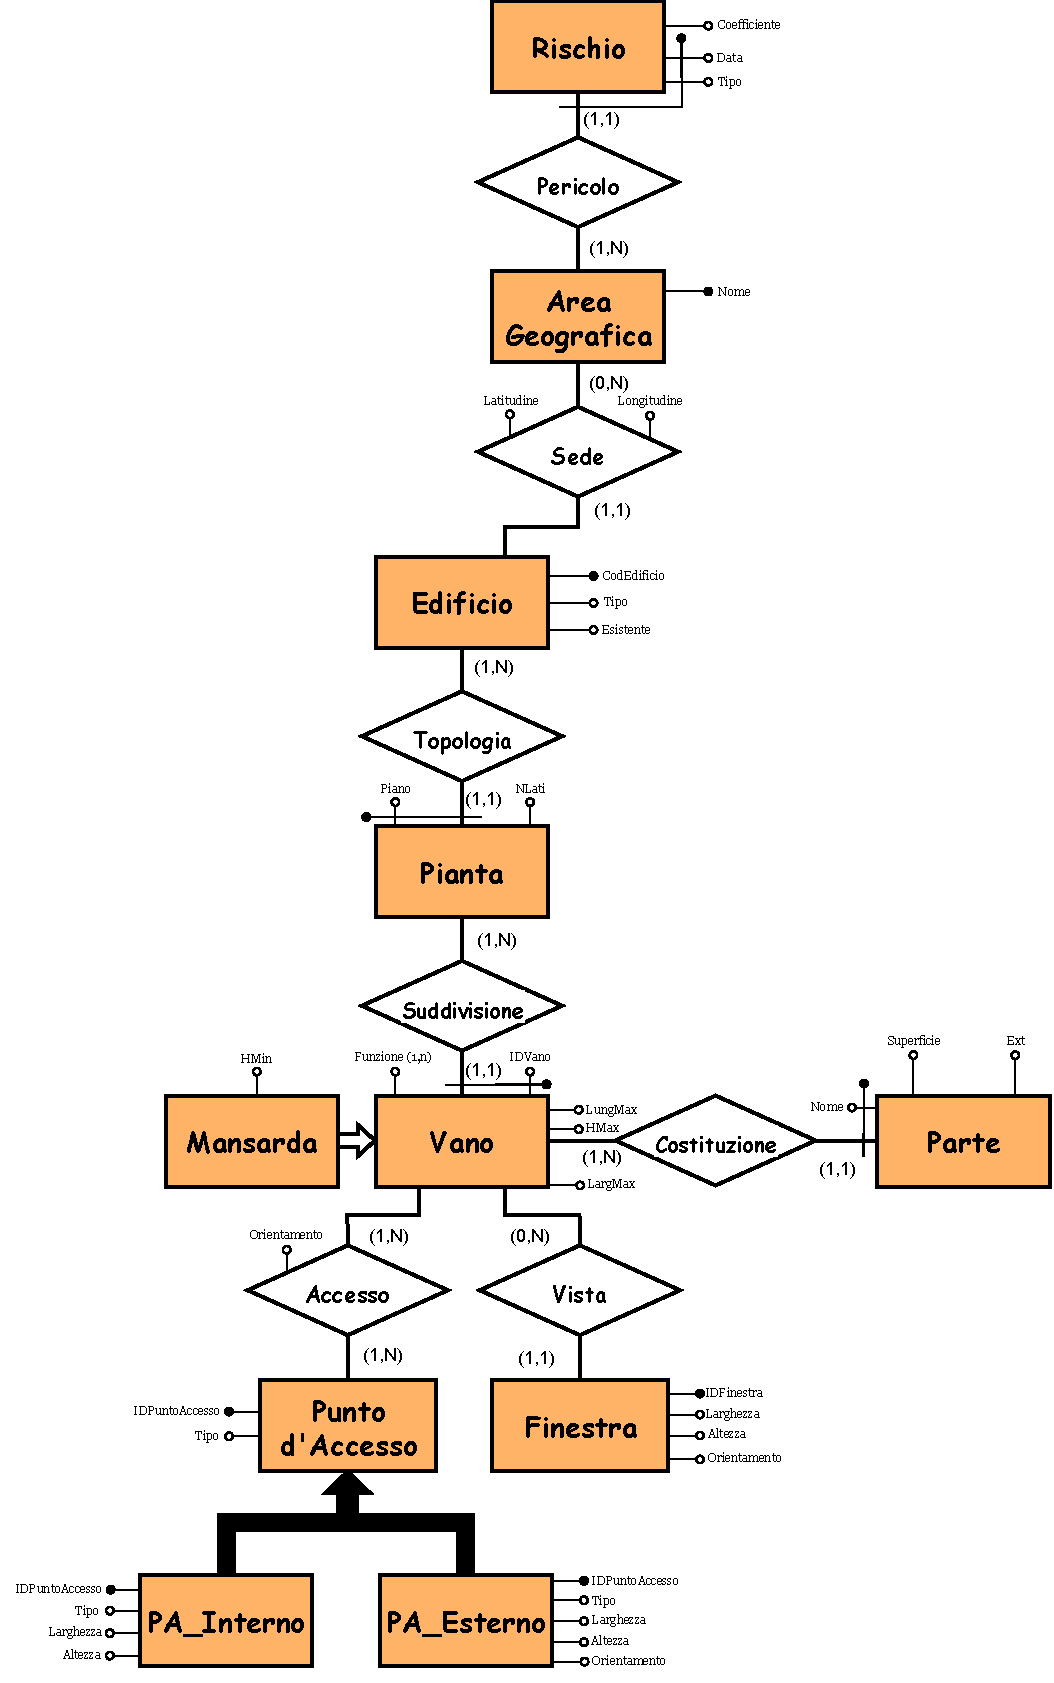
\includegraphics[scale=0.75]{ER_generale.pdf}
    \end{center}
        \section{Struttura di un Edificio}
            
            La parte di diagramma in questione ha lo scopo di descrivere un edificio dal punto di vista 
            strutturale. L'utente può inserire un nuovo edificio, esistente o non, fornendo il suo codice
            identificativo di edificio.

            Saranno inoltre salvate informazioni riguardo alla topologia dell'edificio stesso: la pianta
            di ogni piano; i vani (mansardati o non) che la compongono; e 
            i vari punti d'accesso interni o esterni.

            Le piante delle quali si vogliono memorizzare informazioni devono essere poligonali, il cui numero di lati è anch'esso 
            salvato nella base di dati.

            Un vano deve avere dimensioni massime rappresentate dagli attributi \emph{hMax, lungMax, largMax}. Nel caso in cui il vano sia mansardato, l'attributo \emph{hMin} definisce l'altezza minima del locale.

            Possono essere salvate nel database anche le finestre all'interno di ogni vano, comprensive di dimensioni e orientamento cardinale.

        \section{Rischi}
            Il database salva informazioni riguardanti un rischio di una certa area geografica. 
            
            Del rischio in questione viene salvata la data, l'area geografica alla quale appartiene, un coefficiente, e il tipo di rischio che lo descrive.

            È di grande importanza salvare questo tipo di informazioni nel database affinchè si riesca a determinare un certo rischio a seguito di una esposizione ad un certo pericolo; e il pericolo nel nostro caso è determinato dalla naturale esposizione a calamità.

            Tali calamità saranno esclusivamente di tipo sismico oppure idrogeologico.
    
\chapter{Area Costruzione}
        \begin{center}
            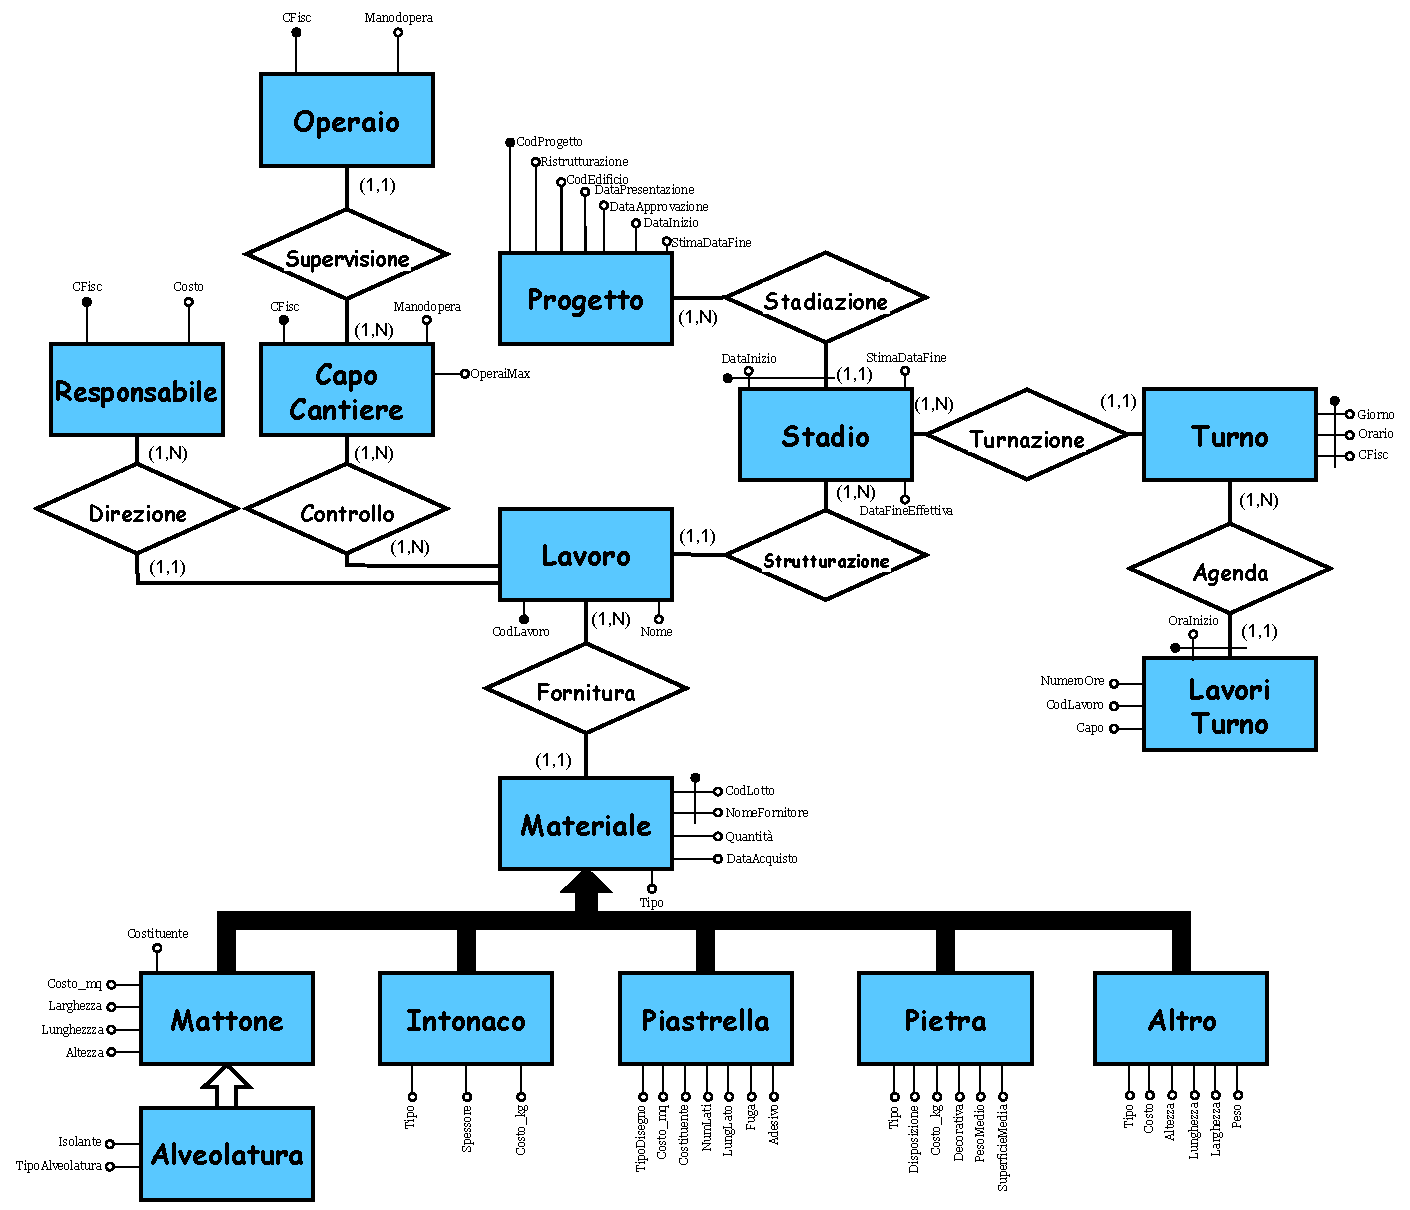
\includegraphics[scale=0.78]{ER_costruzione.pdf}
        \end{center}
        \newpage
        \section{Materiali}
            Parte fondamentale per uno scopo come quello di \emph{Smart Buildings} è memorizzare di quale materiale è fatta una certa parte.

            Alcuni di questi materiali possono essere mattoni, intonaco, piastrelle e pietre. Ciascuno di essi presenta delle caratteristiche individuali, come per esempio lo spessore per un particolare intonaco piuttosto che il tipo di disegno che è presente su una piastrella, e delle caratteristiche comuni come la data di acquisto o il nome del fornitore che li ha venduti.

            Inoltre è presente la possibilità di salvare dei materiali che non sono fra quelli citati sopra, e per farlo gli sono state fornite alcune caratteristiche generali che possono caratterizzare una maggior parte di  materiali in commercio.
        \section{Stadi di Avanzamento e Gestione del Personale}
            I diversi stadi di avanzamento possono essere memorizzati al fine di gestire ogni aspetto di un intero progetto in fase di lavorazione. In effetti il ruolo centrale di questa area della base di dati viene svolto dalle entità Progetto e Lavoro, che insieme ad altri componenti possono contribuire alla memorizzazione di informazioni utili ai fini dell'azienda.
            
            In particolare uno Stadio potrà essere dilazionato in vari ``step'' chiamati Lavoro, e caratterizzati da un codice univoco denominato CodLavoro.

            Riferendoci ora al Lavoro, possiamo dire che per portarlo a termine occorrerà rifornirsi di materiali, i quali sono già stati esplicati nel paragrafo precedente. Per portare a termine un Lavoro occorre anche avere una sezione che riesca a gestire il personale addetto alla manodopera, alla direzione e al monitoraggio.

            Per gestire un personale ampio, dobbiamo memorizzare informazioni su Turno, caratterizzati dal codice fiscale del lavoratore, dal tipo di turno (potenzialmente mattutino o pomeridiano), e dal giorno. Queste informazioni ci permettono di gestire le mansioni che ogni individuo deve svolgere, ma non quali lavori precisamente porterà a termine.

            La memorizzazione dei Lavori all'interno di un turno sarà delegata ad una entità denominata Lavori Turno, che si occuperà di memorizzare l'orario, il codice univoco del lavoro, l'orario di inzio e il numero di ore del Lavoro.

            Per quanto rigurarda le risorse umane, saranno categorizzate come Capo Cantiere, Responsabile o Operaio. Ognuno di essi avrà delle caratteristiche che ci permetteranno di ricercare tutto il personale che compone una unità di lavoro: ovvero dei Capi Cantiere, un Responsabile e un certo numero di operai sotto il monitoraggio (nei limiti dell'esperienza) di un Capo Cantiere. 
    
\chapter{Area Monitoraggio}
        \begin{center}
            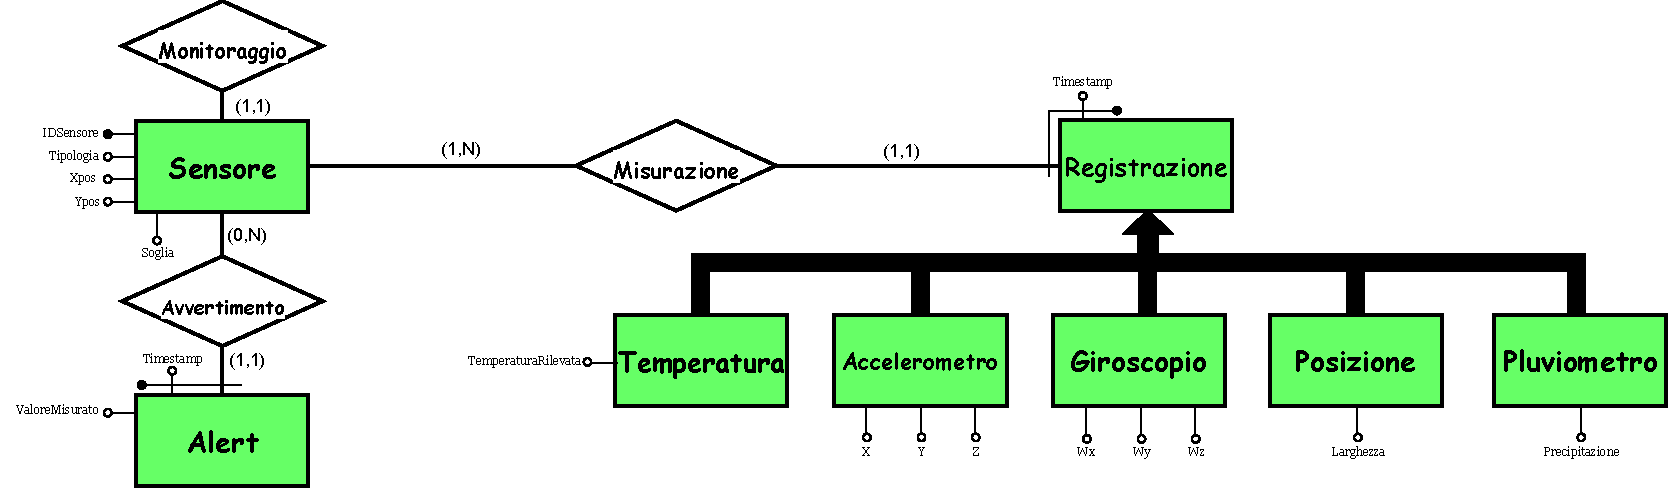
\includegraphics[scale=0.65]{ER_monitoraggio.pdf}
        \end{center}
        \section{Sensoristica}
            La sensoristica ci permette di avere delle rilevazioni senza le quali non potremmo effettuare delle verifiche per testare il malfunzionamento o la previsione di certi eventi, e l'unità fondamentale che ne deriva è un Sensore.

            Il Sensore, ai fini del database, è interpretabile semplicemente come un dispositivo elettronico che permette di misurare delle grandezze fisiche di vario tipo, come la temperatura, o il livello di precipitazioni atmosferiche. Un sensore è quindi identificato da un ID dal quale è possibile risalire alla parte che esso monitora.

        \section{Memorizzazione dei Dati}
        
            La memorizzazione a suo modo collabora al monitoraggio stoccando le misurazioni dei sensori in apposite sezioni del database. Per farlo si serve di Registrazioni, ovvero delle misurazioni di un sensore in un certo istante denominato Timestamp.

            Le Registrazioni tuttavia non offrono un vero riscontro dal punto di vista della sicurezza, perchè una registrazione non è altro che una neutra misurazione della realtà intorno al sensore.

            Gli Alert sono invece delle misurazioni di un certo sensore, che quindi è possibile identificare univocamente, che riportano un valore misurato che potrebbe essere causa di problemi di qualche tipo, come una crepa nel muro.
    
\chapter{Area Analisi del Rischio}
        \begin{center}
            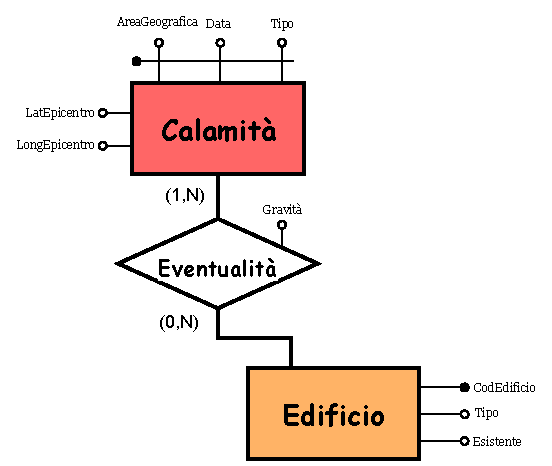
\includegraphics{ER_calamita.pdf}
        \end{center}
        Quest'area risulta fondamentale al momento dell'effettivo istante in cui una Calamità si presenta. La presente sezione del Database si prefissa di salvare le informazioni riguardanti la relazione che c'è fra gli Edifici e le Calamità avvenute, al fine di riuscire a stimare i possibili danni, oppure prevedere tali danni.
        
        Come si può notare, la relazione Eventualità presenta un attributo \emph{Gravita}, che ci permette di associare ad ogni Edificio un indie di gravità in corrispondenza dell'evento Calamitoso preso in considerazione.

        Per semplicità, e considerando i termini didattici dell'elaborato, consideriamo il caso in cui una Calamità di un certo \emph{Tipo}, ovvero \emph{Sismica} oppure \emph{Idrogeologica}, non possa verificarsi all'interno della giornata per più volte.

        Le Calamità e gli Edifici sono identificati geograficamente da \emph{Latitudine} e \emph{Longitudine}. In questo modo è possibile calcolare l'attributo \emph{Gravita} rendendolo dipendente dalla distanza dell'Edificio dall'Evento Calamitoso.
\part{Ristrutturazione}

    \chapter{Eliminazione delle Generalizzazioni}
        \section{Generalizzzione di Vano}
            \label{ref1}
            La generalizzazione parziale Mansarda rappresenta logicamente un vano mansardato. La ristrutturazione potrebbe essere fatta introducendo una entità Mansarda e una relazione che lega la Mansarda al Vano.

            Tuttavia una soluzione migliore si ottiene osservando che un Vano può o no essere mansardato. Questo permette di ristrutturare la generalizzazione inserendo un attributo booleano Mansardato all'interno di Vano, e spostando l'attributo $HMin$ di Mansarda su Vano, permettendo così di non introdurre nè l'entità Mansardato nè la relazione che le avrebbe dovute congiungere. Inoltre, possiamo osservare che il booleano \emph{Mansardato} in questo caso è ridondante, perchè possiamo constatare se lo sia o meno semplicemente comparando gli attributi \emph{HMin} e \emph{HMax}: viene quindi eliminato.

            \vspace*{1.5cm}
            \begin{center}
                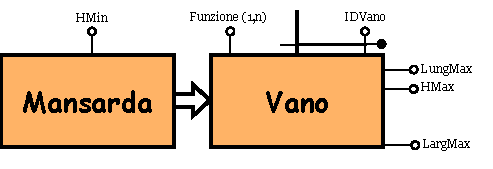
\includegraphics[scale=1.7]{genVano.pdf}
            \end{center}
            \vspace*{1.5cm}
            \begin{center}
                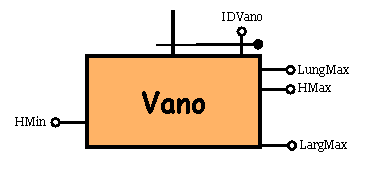
\includegraphics[scale=1.7]{genVanoTrad.pdf}
            \end{center}

            \newpage
            
            \section{Generalizzazione di Punto D'Accesso}
                La generalizzazione di Punto d'Accesso, entità che rappresenta un arco, una porta, una portafinestra o simili, è di tipo totale, perchè l'eventualità che un Punto d'Accesso possa essere Interno, esclude completamente il caso in cui possa essere contemporaneamente Esterno.
                \begin{center}
                    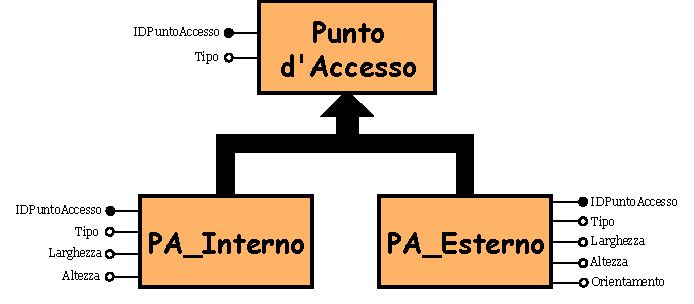
\includegraphics[scale=1.1]{genPuntoAccesso.pdf}
                \end{center}
                \vspace*{0.5cm}
                La ristrutturazione è stata effettuata per mezzo di due entità: AccessoI e AccessoE. 
                
                Per quanto riguarda i Punti di Accesso Esterni, possono essere presenti oppure no, infatti esistono Vani la cui posizione li costringe ad essere circondati da altri Vani, dunque parteciperà opzionalmente in AccessoE. 
                
                Nel caso dei Punti di Accesso Interni la soluzione è leggermente più complessa. Infatti ci troviamo davanti ad una relazione ``molti a molti", perchè un Punto di Accesso Interno collegherà necessariamente due Vani, e allo stesso tempo un Vano ne può avere più di uno. La soluzione prevede che i Punti di Accesso Interni abbiano un identificatore univoco $IDPuntoAccesso$ che li identifica, e che in AccessoI ci sia salvato l'orientamento del Punto di Accesso Interno di tale Vano. In questa logica, se ad esempio avessimo due Vani comunicanti tramite una porta, avremo una tupla che identifica che quella porta si trova in un certo punto cardinale di un Vano, mentre in un'altra tupla avremo che la stessa porta nel Vano adiacente si troverà orientata al contrario.
                \vspace*{0.5cm}
                \begin{center}
                    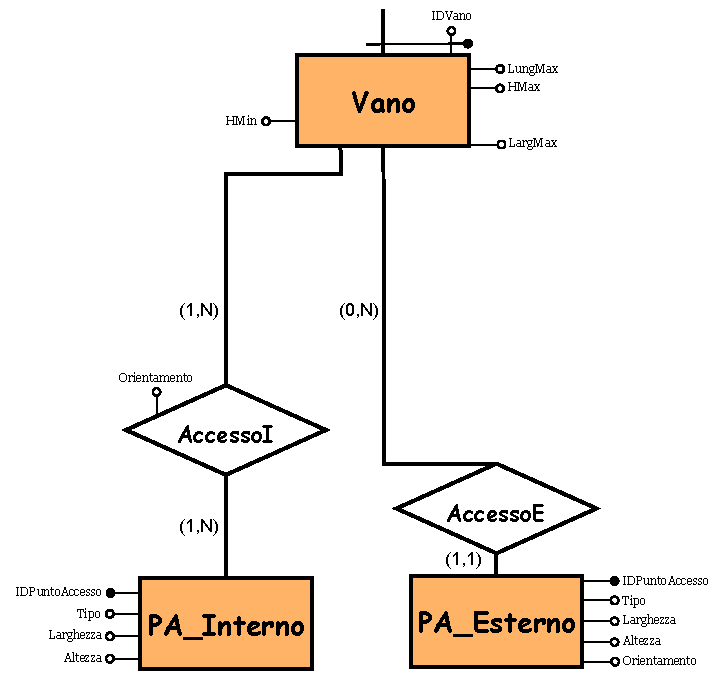
\includegraphics[scale=0.9]{genPuntoAccessoTrad.pdf}
                \end{center}
            \section{Generalizzazione di Materiale}
            \label{ref2}
                \begin{center}
                    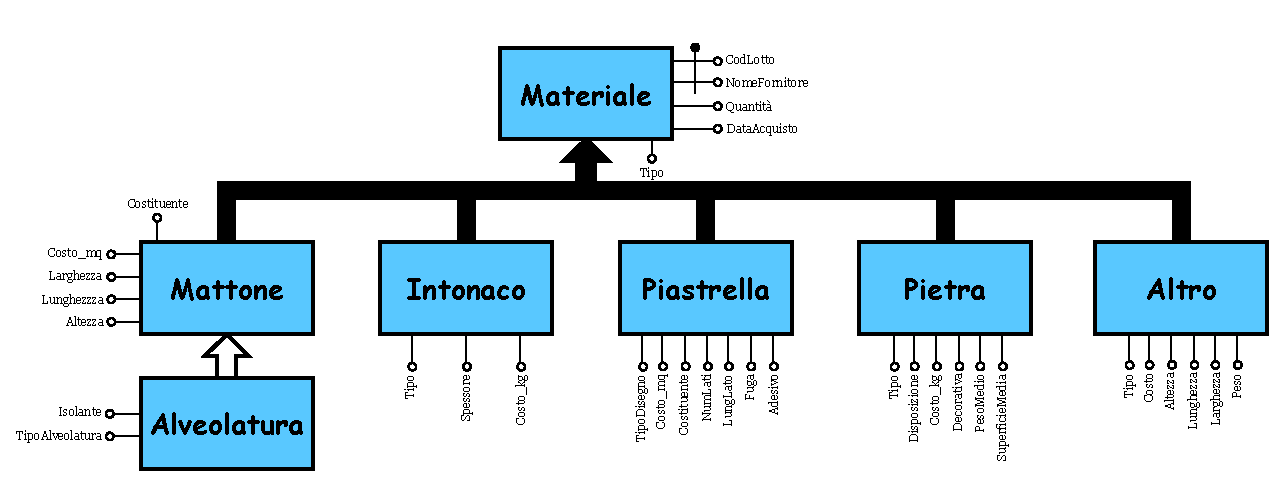
\includegraphics[scale=0.8]{genMateriale.pdf}
                \end{center}
                \vspace*{0.8cm}
                La generalizzazione di Materiale è stata ristrutturata considerando che un elemento dell'entità Materiale rappresenta un Lotto, che quindi sarà costituito da un solo materiale. Fatta questa assunzione, e considerato che le entità derivate da Materiale hanno tutte attributi molto diversi, la soluzione adottata è stata quella di tenere i figli e legarli dalle rispettive relazioni facoltative che permettono di accedere alle informazioni grazie alla chiave esterna che ognuna di loro ha nei confronti di Materiale.

                \vspace*{0.8cm}
                \begin{center}
                    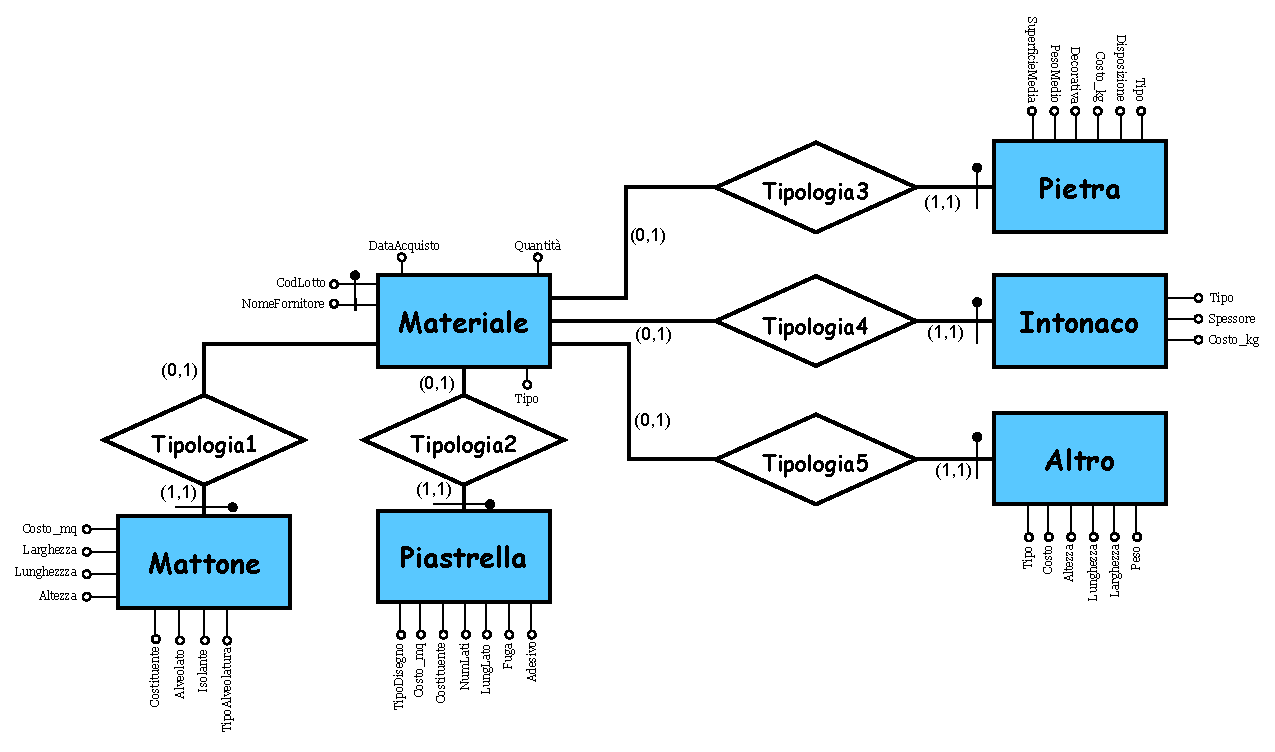
\includegraphics[scale=0.8]{genMaterialeTrad.pdf}
                \end{center}
                \vspace*{0.8cm}
                
                C'è da precisare che anche la generalizzazione parziale di Mattone e Alveolatura è stata gestita esattamente come in precedenza è stata gestita la generalizzazione tra Vano e Mansarda, si omettono quindi considerazioni ridondanti (\ref{ref1}).
                
                \section{Generalizzazione di Registrazione}
                \vspace*{1cm}
                \begin{center}
                    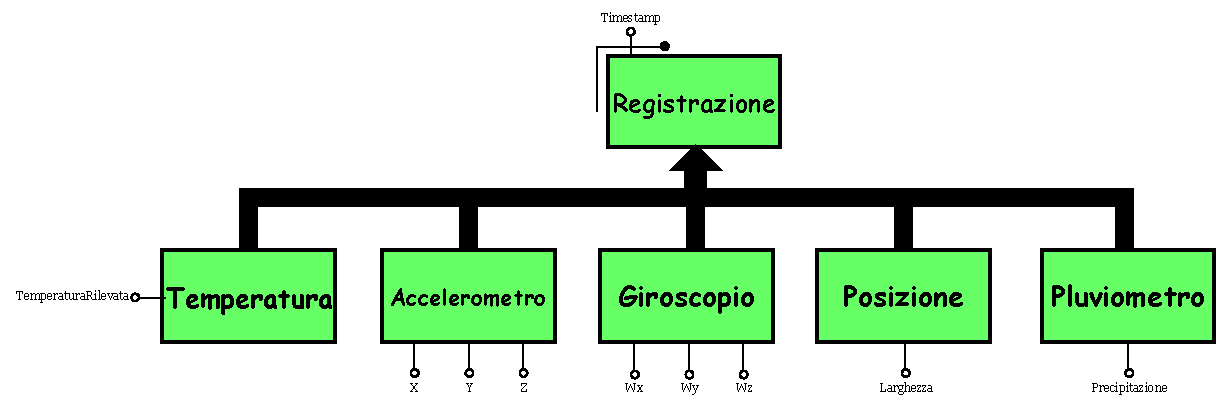
\includegraphics[scale=0.8]{genRegistrazione.pdf}
                \end{center}
                \vspace*{1cm}
                Le stesse cosiderazioni fatte per la generalizzazione totale precedente (\ref{ref2}) possono essere fatte anche in questo caso. Di nuovo gli attributi sono molto diversi fra i figli, e l'accesso avviene in una sola delle entità figlie, perchè l'esistenza di una tupla del padre implica l'esistenza di una sola tupla relativa ai figli. La ristrutturazione quindi risulta essere la seguente.
                \vspace*{1cm}
                \begin{center}
                    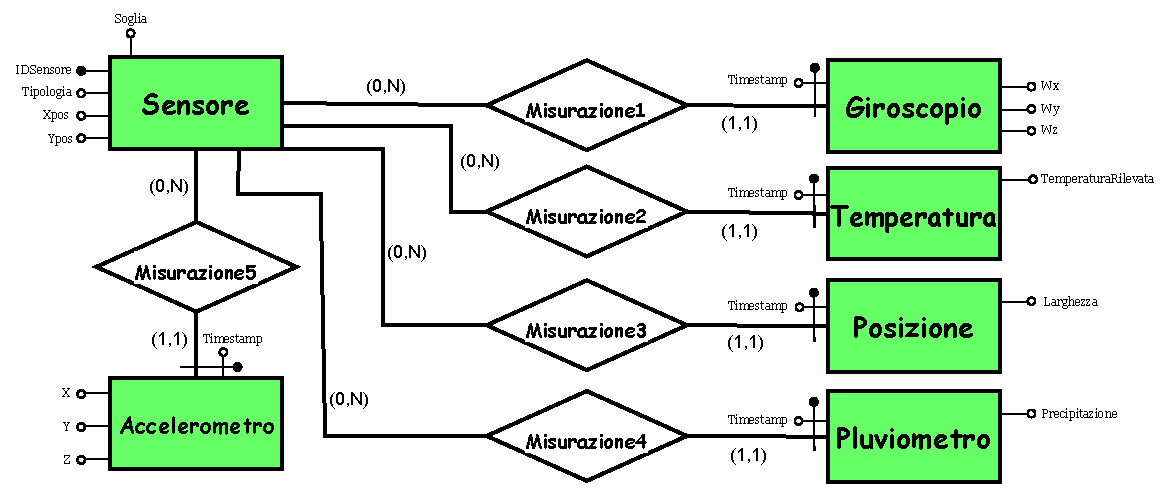
\includegraphics[scale=0.9]{genRegistrazioneTrad.pdf}
                \end{center}
                
                \chapter{Eliminazione di attributi multivalore}
                \section{Attributo multivalore Funzione}
                \begin{center}
                    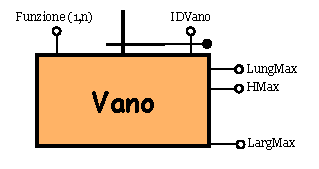
\includegraphics[scale=1.3]{multiFun.pdf}
                \end{center}
                \vspace*{1cm}
                La necessità dell'attributo multivalore Funzione nasce dalla possibilità di un Vano di poter avere più di una funzione.
                
                \vspace*{1cm}
            \begin{multicols}{2}
                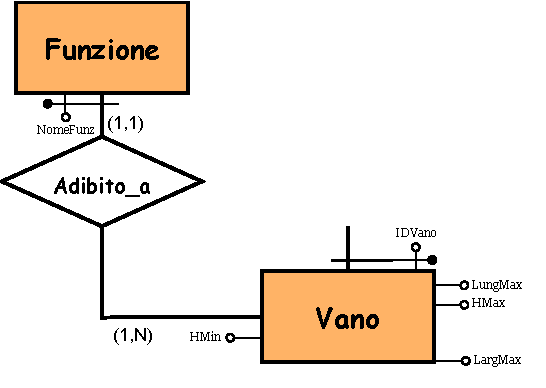
\includegraphics[scale=1.0]{multiFunTrad.pdf}
                Questa casistica ci porta necessariamente a rimuovere l'attributo multivalore introducendo una entità Funzione e una relazione Adibito\_a. Nella soluzione adottata, la funzione appartiene ad un solo Vano, ma un Vano può avere più Funzioni. In questo modo per ogni tupla di Vano esisterà almeno una tupla Funzione che fa riferimento a quello specifico Vano.
            \end{multicols}

\part{Analisi Prestazionale}

    \chapter{Tavola dei Volumi}
        \begin{center}
            \begin{tabular}{|p{4cm}|p{1cm}|p{3cm}|p{8cm}|}
                \hline
                \rowcolor{celeste}\multicolumn{4}{|c|}{\textbf{Area Costruzione}} \\ \hline
                \textbf{Concetto} & \textbf{Tipo} & \textbf{Volume} & \textbf{Considerazioni} \\ \hline
                Materiale & E & 3*1.080 = 3.240 & Ipotizzando che una Parte sia composta mediamente da 3 materiali \\ \hline
                Mattone & E & 0,2*1.080 = 216 & Ipotizzando che il 20\% dei Materiali siano Mattone \\ \hline
                Piastrella & E & 0,2*1.080 = 216 & Ipotizzando che il 20\% dei Materiali siano Piastrella \\ \hline
                Pietra & E & 0,2*1.080 = 216 & Ipotizzando che il 20\% dei Materiali siano Pietra \\ \hline
                Intonaco & E & 0,3*1.080 =  324 & Ipotizzando che il 30\% dei Materiali siano Intonaco \\ \hline
                Altro & E & 0,1*1.080 = 108 & Ipotizzando che il 10\% dei Materiali siano Altro \\ \hline
                Lavoro & E & 0,5*3.240 = 1.620 & Ipotizzando 2 Materiali per ogni Lavoro \\ \hline
                Capo Cantiere & E & 45 & Ipotizzato \\ \hline
                Operaio & E & 12*45 = 540 & Ipotizzando in media 12 Operai per Capo Cantiere \\ \hline
                Responsabile & E & 2*14 = 28 & Ipotizzando 2 Responsabili per ogni Progetto \\ \hline
                Progetto & E & 10+4 = 14 & Ipotizzando 10 costruzioni e 4 ristrutturazioni \\ \hline
                Stadio & E & 14*3 = 42 & Ipotizzando 3 Stadi per ogni Progetto \\ \hline
                Turno & E & 110.000 & Ipotizzato \\ \hline
                Lavori Turno & E & 440.000 & Ipotizzato \\ \hline
                Composizione & R & 3.240 & Stesso volume di Materiale \\ \hline
                Tipologia 1 & R & 216 & Stesso volume di Mattone \\ \hline
                Tipologia 2 & R & 216 & Stesso volume di Piastrella \\ \hline
                Tipologia 3 & R & 216 & Stesso volume di Pietra \\ \hline
                Tipologia 4 & R & 324 & Stesso volume di Intonaco \\ \hline
                Tipologia 5 & R & 108 & Stesso volume di Altro \\ \hline
                Fornitura & R & 3.240 & Stesso volume di Materiale \\ \hline
                Controllo & R & 1,3*1.620 = 2.106 & Ipotizzando 1,3 Capi Cantiere per ogni Lavoro \\ \hline
                Supervisione & R & 540 & Stesso volume di Operaio \\ \hline
                Direzione & R & 1.620 & Stesso volume di Lavoro \\ \hline
                Stadiazione & R & 42 & Stesso volume di Stadio \\ \hline
                Strutturazione & R & 1.620 & Stesso volume di Lavoro \\ \hline
                Turnazione & R & 110.000 & Stesso volume di Turno \\ \hline
                Agenda & R & 440.000 & Stesso volume di Lavori Turno \\ \hline
            \end{tabular}
            
            \begin{tabular}{|p{4cm}|p{1cm}|p{3cm}|p{8cm}|}
                \hline
                \rowcolor{rosso}\multicolumn{4}{|c|}{\textbf{Area Analisi Rischio}} \\ \hline
                \textbf{Concetto} & \textbf{Tipo} & \textbf{Volume} & \textbf{Considerazioni} \\ \hline
                Calamità & E & 6 & Ipotizzato \\ \hline
                Eventualità & R & 8 & Ipotizzato \\ \hline
            \end{tabular}
            
            \begin{tabular}{|p{4cm}|p{1cm}|p{3cm}|p{8cm}|}
                \hline
                \rowcolor{giallo}\multicolumn{4}{|c|}{\textbf{Area Generale}} \\ \hline
                \textbf{Concetto} & \textbf{Tipo} & \textbf{Volume} & \textbf{Considerazioni} \\ \hline
                Rischio & E & 3*5 = 15 & Ipotizzando mediamente 3 rischi per area \\ \hline
                Area Geografica & E & 5 & Ipotizzato \\ \hline
                Edificio & E & 10 & Ipotizzato \\ \hline
                Funzione & E & 1,2*180 = 216 & Ipotizzando 12 funzioni ogni 10 vani \\ \hline
                Pianta & E & 3*10 = 30  & Ipotizzando mediamente 3 piani per edificio \\ \hline
                Vano & E & 6*30 = 180 & Ipotizzando mediamente 6 vani per pianta \\ \hline
                Finestra & E & 1,3*180  = 234 & Ipotizzando 13 finestre ogni 10 vani \\ \hline
                PA\_Interno & E & 288 & Ipotizzando l'80\% dei punti d'accesso come interni* \\ \hline
                PA\_Esterno & E & 72 & Ipotizzando il 20\% dei punti d'accesso come esterni* \\ \hline
                Parte & E & 6*180 = 1.080 & Ipotizzando 4 pareti, un soffitto e un pavimento \\ \hline
                Pericolo & R & 15 & Stesso volume di Rischio \\ \hline
                Sede & R & 10 & Stesso volume di Edificio \\ \hline
                Topologia & R & 30 & Stesso volume di Pianta \\ \hline
                Adibito\_a & R & 216 & Stesso volume di Funzione \\ \hline
                Suddivisione & R & 180 & Stesso volume di Vano \\ \hline
                AccessoE & R & 72 & Stesso volume di PA\_Esterno \\ \hline
                AccessoI & R & 288*1,6 = 461 & Supponendo 16 Punti di Accesso Interni ogni 10 Vani \\ \hline
                Vista & R & 234 & Stesso volume di Finestra \\ \hline
                Costituzione & R & 1.080 & Stesso volume di Parte \\ \hline
                \multicolumn{4}{|r|}{*ipotizzando in media 2 punti di accesso per vano, ci sono 360 punti di accesso} \\ \hline
            \end{tabular}
            
            \begin{tabular}{|p{4cm}|p{1cm}|p{3cm}|p{8cm}|}
                \hline
                \rowcolor{verde}\multicolumn{4}{|c|}{\textbf{Area Monitoraggio}} \\ \hline
                \textbf{Concetto} & \textbf{Tipo} & \textbf{Volume} & \textbf{Considerazioni} \\ \hline
                Sensore & E & 310 & Ipotizzato \\ \hline
                Accelerometro & E & 30*3.650 = 109.500 & Ipotizzando un Accelerometro per Piano* \\ \hline
                Giroscopio & E & 30*3.650 = 109.500 & Ipotizzando un Giroscopio per Piano* \\ \hline
                Temperatura & E & 180*3.650 = 657.000 & Ipotizzando un sensore di Temperatura per Vano* \\ \hline
                Posizione & E & 6*10*3.650 = 219.000 & Ipotizzando 6 sensori di Posizione per Edificio* \\ \hline
                Pluviometro & E & 10*3.650 = 36.500 & Ipotizzando un Pluviometro per Edificio* \\ \hline
                Alert & E & 0,3*1.131.500 = 339.450 & Ipotizzando chen il 30\% delle Misurazioni generino un Alert \\ \hline
                Misurazione1 & R & 109.500 & Stesso volume di Giroscopio \\ \hline
                Misurazione2 & R & 657.000 & Stesso volume di Temperatura \\ \hline
                Misurazione3 & R & 219.000 & Stesso volume di Posizione \\ \hline
                Misurazione4 & R & 36.500 & Stesso volume di Pluviometro \\ \hline
                Misurazione5 & R & 109.500 & Stesso volume di Accelerometro \\ \hline
                Monitoraggio & R & 310 & Stesso volume di Sensore \\ \hline
                Avvertimento & R & 339.450 & Stesso volume di Alert \\ \hline
                \multicolumn{4}{|r|}{*ipotizzando 2 misurazioni al giorno per 5 anni} \\ \hline
            \end{tabular}
            
        \end{center}
        
        \chapter{Operazioni sui Dati}
        \section{Operazione 1 - trovaAlert}
        Data una calamità, l'operazione prende in considerazione tutti gli Edifici presenti nell'Area Geografica dove la Calamità ha avuto luogo. Successivamente, per ogni Edificio trovato, trova tutti gli Alert che sono stati generati dalle misurazioni dei Sensori in seguito all'Evento Calamitoso e ne restituisce i dati.
        
        La frequenza presa in esame è di 2 volte all'anno, e tiene in considerazione il fatto che una richiesta del genere probabilmente verrà effettuata un paio di volte in seguito ad un Evento Calamitoso, e che gli Eventi Calamitosi della Tabella dei Volumi sono relativi a 5 anni.
        
        \begin{center}
            \begin{tabular}{|c|c|c|}
                \hline
                \rowcolor{viola} \textbf{Input} & \textbf{Output} & \textbf{Frequenza} \\ \hline
                AreaGeografica, Data, Tipo & CodEdificio, IDSensore e Alert & 2 volte all'anno \\ \hline
            \end{tabular}
        \end{center}
        
        \subsection{Sezione di Diagramma Interessato}
        \begin{center}
            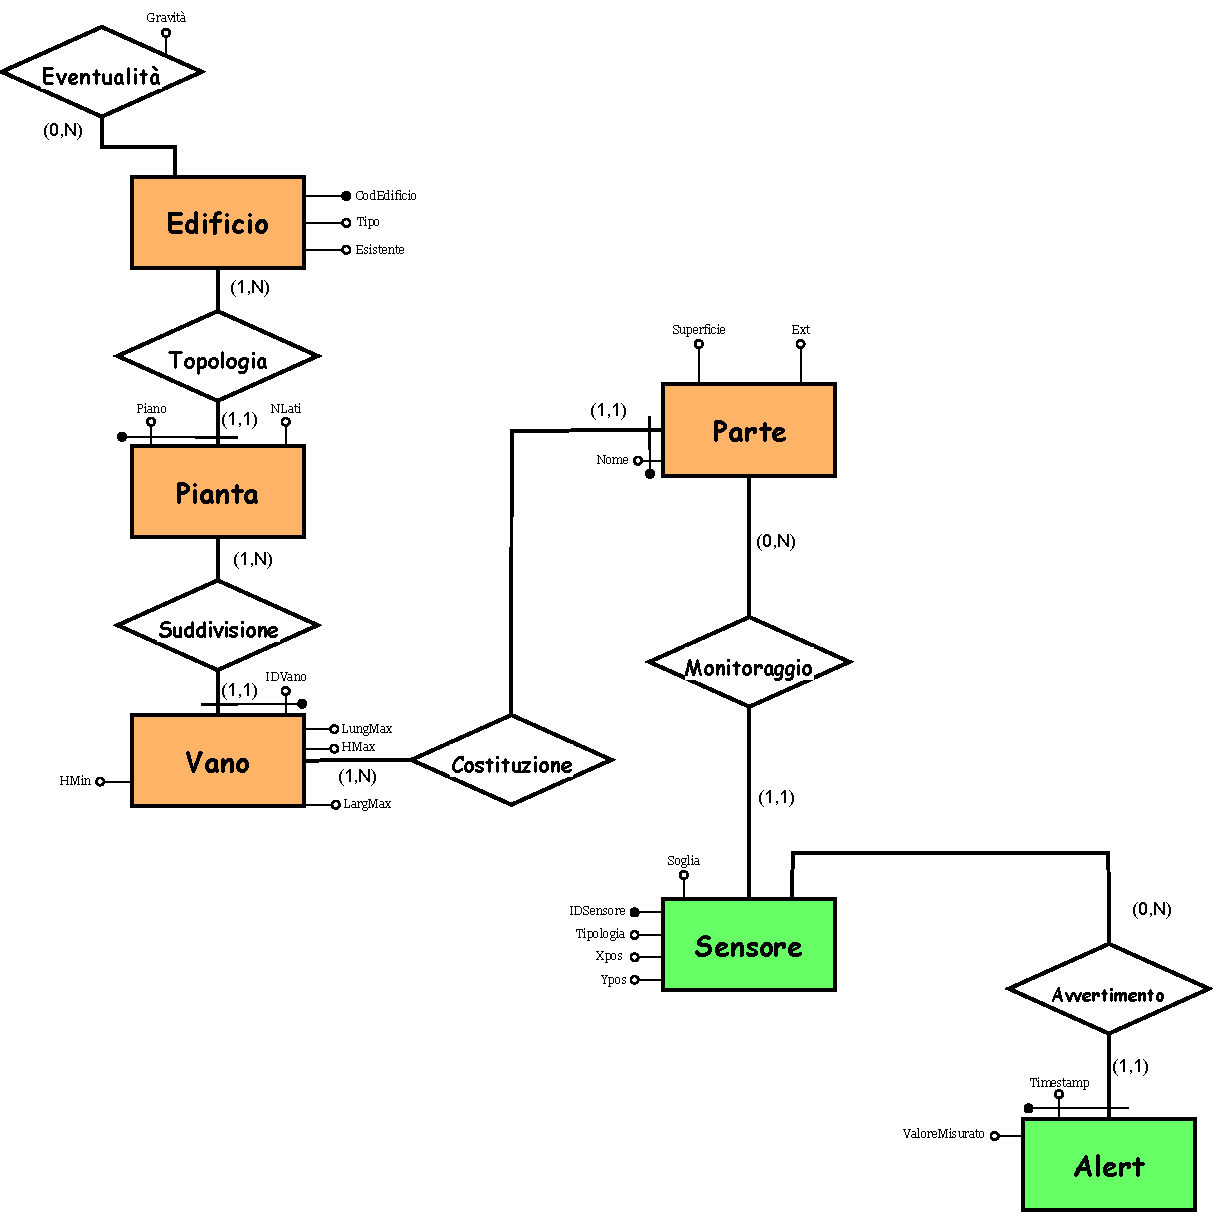
\includegraphics[scale=0.7]{sezione_operazione1.pdf}
        \end{center}
        
        \subsection{Tavola dei Volumi Interessati}
        \begin{tabular}{|p{4cm}|p{1cm}|p{3cm}|p{8cm}|}
            \hline
            \textbf{Concetto} & \textbf{Tipo} & \textbf{Volume} & \textbf{Considerazioni} \\ \hline
            Eventualità & R & 8 & Ipotizzato \\ \hline
            Monitoraggio & R & 310 & Stesso volume di Sensore \\ \hline
            Alert & E & 0,3*1.131.500 = 339.450 & Ipotizzando che il 30\% delle Misurazioni generino un Alert \\ \hline
        \end{tabular}
        
        \subsection{Tavola degli Accessi}
        \begin{tabular}{|c|c|c|c|p{4cm}|p{3.5cm}|c|}
            \hline
            \textbf{id} & \textbf{Concetto} & \textbf{Costrutto} & \textbf{Tipo} & \textbf{Considerazioni} & \textbf{Accessi} & \textbf{Dim(Ris)} \\ \hline
            1 & Eventualità & R & Lettura & Leggo gli edifici colpiti & Vol(Eventualità) = 8 & 2 \\ \hline
            2 & Monitoraggio & R & Lettura & Leggo i sensori degli edifici colpiti dalla Calamità & Vol(Monitoraggio) *2 = 310*2 = 620 & 62 \\ \hline
            3 & Alert & E & Lettura & Leggo gli alert che i sensori hanno generato durante la Calamita & Vol(Alert)*62 = 339.450*62 = 21.045.900 & ~ \\ \hline
            \multicolumn{5}{|c|}{Totale degli accessi per 1 volta} & \multicolumn{2}{|c|}{21.046.528} \\ \hline
            \multicolumn{5}{|c|}{Totale degli accessi per 2 volte} & \multicolumn{2}{|c|}{21.046.528*2 = 42.093.056} \\ \hline
        \end{tabular}

        \newpage

        \section{Operazione 2 - topologiaEdificio}
        Dato il codice di un Edificio, l'operazione restituisce tutte le informazioni necessarie per poter riprodurre fedelmente ``su carta" la pianta dell'Edificio preso in considerazione. In particolare l'output consiste in tutti i valori degli attributi di tutte le entità Pianta e Vano.
        
        Possiamo considerare la frequenza dell'operazione di circa 2 volte alla settimana, tenendo presente che potrebbe servire al personale addetto per tenere sotto controllo i lavori, oppure fornire su richiesta la pianta in versione grafica.
        
        \begin{center}
            \begin{tabular}{|c|c|c|}
                \hline
                \rowcolor{viola} \textbf{Input} & \textbf{Output} & \textbf{Frequenza} \\ \hline
                CodEdificio & Vani, Piante, Punti d'Accesso e Finestre & 2 volte a settimana \\ \hline
            \end{tabular}
        \end{center}
        
        \subsection{Sezione di Diagramma Interessato}
        \begin{center}
            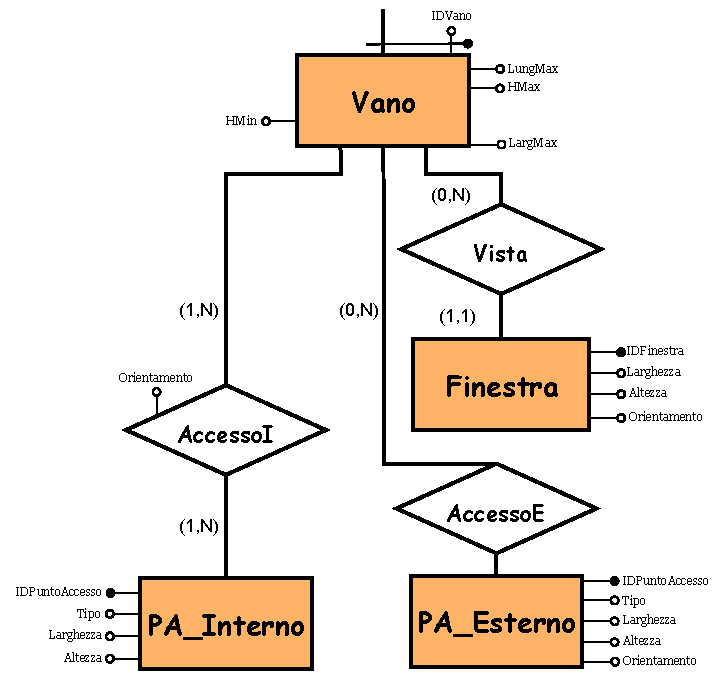
\includegraphics[scale=1.45]{sezione_operazione2.pdf}
        \end{center}
        
        \subsection{Tavola dei Volumi Interessati}
            \begin{tabular}{|p{4cm}|p{1cm}|p{3cm}|p{8cm}|}
                \hline
                \textbf{Concetto} & \textbf{Tipo} & \textbf{Volume} & \textbf{Considerazioni} \\ \hline
                Vano & E & 6*30 = 180 & Ipotizzando mediamente 6 vani per pianta \\ \hline
                AccessoI & R & 288*1,6 = 461 & Supponendo 16 Punti di Accesso Interni ogni 10 Vani \\ \hline
                PA\_Interno & E & 288 & Ipotizzando l'80\% dei punti d'accesso come interni* \\ \hline
                AccessoE & R & 72 & Stesso volume di PA\_Esterno \\ \hline
                PA\_Esterno & E & 72 & Ipotizzando il 20\% dei punti d'accesso come esterni* \\ \hline
                Vista & R & 234 & Stesso volume di Finestra \\ \hline
                Finestra & E & 1,3*180 = 234 & Ipotizzando 13 finestre ogni 10 vani \\ \hline
                \multicolumn{4}{|l|}{* ipotizzando in media 2 punti di accesso per vano, ci sono 360 punti di accesso} \\ \hline
            \end{tabular}
        
        \subsection{Tavola degli Accessi}
        \begin{tabular}{|c|c|c|c|p{4cm}|p{3cm}|c|}
            \hline
            \textbf{id} & \textbf{Concetto} & \textbf{Costrutto} & \textbf{Tipo} & \textbf{Considerazioni} & \textbf{Accessi} & \textbf{Dim(Ris)} \\ \hline
            1 & Vano & E & Lettura & Leggo i vani dell'edificio & Vol(Vano) = 180 & 18 \\ \hline
            2 & AccessoI & R & Lettura & Leggo IDPuntoAccesso e Orientamento & Vol(Accesso\_I) * 18 = 461 * 18 = 8.298 & 29 \\ \hline
            3 & PA\_Interno & E & Lettura & Leggo il Tipo & 29 & ~ \\ \hline
            4 & AccessoE & R & Lettura & Leggo IDPuntoAccesso & Vol(AccessoE) * 18 = 72 * 18 = 1.296 & 7 \\ \hline
            5 & PA\_Esterno & E & Lettura & Leggo le informazioni che mi servono & 7 & ~ \\ \hline
            6 & Vista & R & Lettura & Leggo IDFinestra & Vol(Vista)*18 = 234*18 = 4.212 & 1,3*18 = 23 \\ \hline
            7 & Finestra & E & Lettura & Leggo le informazioni che mi servono & 23 & ~ \\ \hline
            \multicolumn{5}{|c|}{Totale degli accessi per 1 volta} & \multicolumn{2}{|c|}{14.045} \\ \hline
            \multicolumn{5}{|c|}{Totale degli accessi per 2 volte} & \multicolumn{2}{|c|}{14.045*2 = 28.090} \\ \hline
        \end{tabular}
        
        \newpage

        \section{Operazione 3 - rischiAnnui}
        Dato in input il codice di un Edificio, l'operazione ha lo scopo di riuscire ad analizzare le correlazioni che esistono, all'interno dell'anno attuale, fra i Coefficienti di Rischio che riguardano l'area geografica dove ha sede quell'Edificio. Quello che restituisce risulta essere l'insieme delle informazioni necessarie alla valutazione. Un'operazione del genere può risultare fondamentale nell'analisi preventiva degli edifici e nella risoluzione preventiva di futuri possibili malfunzionamenti.
        
        Per quanto riguarda la stima della frequenza per questa operazione, possiamo considerare di richiamarla stagionalmente, e quindi moltiplicando per quattro il volume di Edificio si arriva ad una frequenza annua di 40 volte.
        
        \begin{center}
            \begin{tabular}{|c|c|c|}
                \hline
                \rowcolor{viola} \textbf{Input} & \textbf{Output} & \textbf{Frequenza} \\ \hline
                CodEdificio & Rischio & 40 volte all'anno \\ \hline
            \end{tabular}
        \end{center}
        
        \subsection{Sezione di Diagramma Interessato}
        \begin{center}
            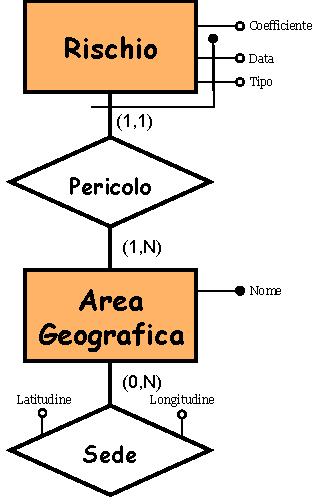
\includegraphics{sezione_operazione3.pdf}
        \end{center}
        
        \subsection{Tavola dei Volumi Interessati}
        \begin{tabular}{|p{4cm}|p{1cm}|p{3cm}|p{8cm}|}
            \hline
            \textbf{Concetto} & \textbf{Tipo} & \textbf{Volume} & \textbf{Considerazioni} \\ \hline
            Sede & R & 10 & Stesso volume di Edificio \\ \hline
            Rischio & E & 3 * 5 = 15 & Ipotizzando mediamente 3 rischi per area \\ \hline
        \end{tabular}
        
        \subsection{Tavola degli Accessi}
        \begin{tabular}{|c|c|c|c|p{4cm}|p{3cm}|c|}
            \hline
            \textbf{id} & \textbf{Concetto} & \textbf{Costrutto} & \textbf{Tipo} & \textbf{Considerazioni} & \textbf{Accessi} & \textbf{Dim(Ris)} \\ \hline
            1 & Sede & R & Lettura & Leggo la sede dell'Edificio & 1 & 1 \\ \hline
            2 & Rischio & R & Lettura & Leggo tutti i rischi e confronto i coefficienti & Vol(Rischio)*1 = 15*1 = 15 & 15 \\ \hline
            \multicolumn{5}{|c|}{Totale degli accessi per 1 volta} & \multicolumn{2}{|c|}{16} \\ \hline
            \multicolumn{5}{|c|}{Totale degli accessi per 40 volte} & \multicolumn{2}{|c|}{16*40 = 640} \\ \hline
        \end{tabular}
        

        \section{Operazione 4 - leggiBustaPaga}
            L'operazione, che prende in input il codice fiscale di un Operaio, si pone l'obiettivo di calcolarne lo stipendio del mese in corso.
            Come si puo' evincere, la frequenza con la quale viene richiamata e' stimata mensilmente come il numero degli operai presenti nella Base di Dati.

            \begin{center}
                \begin{tabular}{|c|c|c|}
                    \hline
                    \rowcolor{viola} \textbf{Input} & \textbf{Output} & \textbf{Frequenza} \\ \hline
                    CFisc (di un Operaio) & Scalare di tipo Float & Vol(Operaio) = 540 volte al mese \\ \hline
                \end{tabular}
            \end{center}
            
            \subsection{Sezione di Diagramma Interessato}
            \begin{center}
                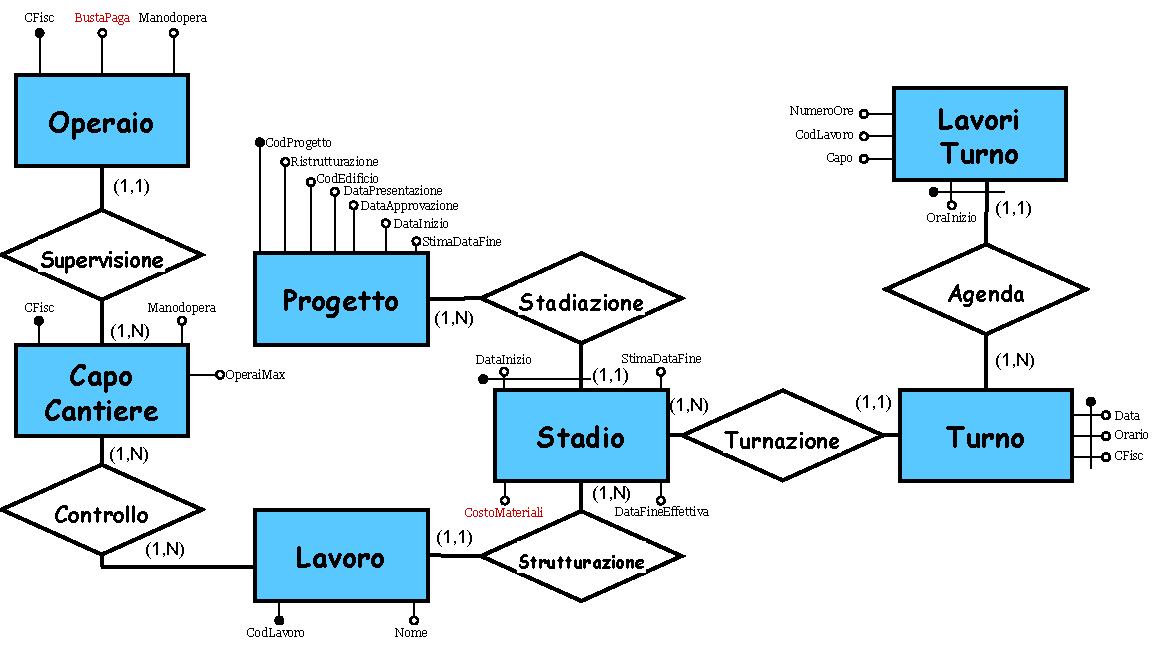
\includegraphics[scale=0.95]{sezione_operazione4.pdf}
            \end{center}
            
            \subsection{Tavola dei Volumi Interessati}
            \begin{tabular}{|p{4cm}|p{1cm}|p{3cm}|p{8cm}|}
                \hline
                \textbf{Concetto} & \textbf{Tipo} & \textbf{Volume} & \textbf{Considerazioni} \\ \hline
                Lavori Turno & E & 440.000 & Ipotizzato \\ \hline
                Operaio & E & 12*45 = 540 & Ipotizzando in media 12 Operai per Capo Cantiere \\ \hline
            \end{tabular}
            
            \subsection{Tavola degli Accessi}
            \begin{tabular}{|c|c|c|c|p{4cm}|p{3cm}|c|}
                \hline
                \textbf{id} & \textbf{Concetto} & \textbf{Costrutto} & \textbf{Tipo} & \textbf{Considerazioni} & \textbf{Accessi} & \textbf{Dim(Ris)} \\ \hline
                1 & Operaio & E & Lettura & Leggo la Manodopera dell'operaio & 1 & 1 \\ \hline
                2 & LavoriTurno & E & Lettura & Sommo le ore lavorative nel mese e le moltiplico per la Manodopera & Vol(LavoriTurno) = 440.000 & ~ \\ \hline
                \multicolumn{5}{|c|}{Totale degli accessi per 1 volta mensile} & \multicolumn{2}{|c|}{440.001} \\ \hline
                \multicolumn{5}{|c|}{Totale degli accessi per 540 volte mensili} & \multicolumn{2}{|c|}{440.001*540 = 237.600.540} \\ \hline
            \end{tabular}

            \subsection{Valutazione della Ridondanza BustaPaga in Operaio}
            Dato l'elevato numero di accessi necessari per portare a termine l'operazione, si decide di valutare l'inserimento di una ridondanza che possa diminuirlo. In particolare si è deciso di valutare la ridondanza BustaPaga come attributo dell'entità Operaio. In questo modo, all'inserimento di ogni tupla in LavoriTurno, si aggiorna la ridondanza per poi effettuare meno accessi nel momento della chiamata all'operazione.

            Come detto in precedenza, la Tavola dei Volumi si riferisce a 5 anni di attività della Base di Dati, occorre quindi stimare il numero dei nuovi Lavori presenti nell'entità LavoriTurno ogni anno. Questa stima può essere fatta dividendo il numero di tuple presente in LavoriTurno per 5, che rappresentano gli anni, e successivamente per 12, che rappresentano i mesi in un anno, ottenedo quindi 7333 nuove tuple in LavoriTurno al mese.

            \subsubsection{Tavola degli Accessi con Ridondanza}
            \begin{tabular}{|c|c|c|c|p{4cm}|p{3cm}|c|}
                \hline
                \textbf{id} & \textbf{Concetto} & \textbf{Costrutto} & \textbf{Tipo} & \textbf{Considerazioni} & \textbf{Accessi} & \textbf{Dim(Ris)} \\ \hline
                1 & Operaio & E & Lettura & Leggo la BustaPaga & 540 & ~ \\ \hline
                2 & Operaio & E & Scrittura & Azzero la BustaPaga del mese scorso & 540 & ~ \\ \hline
                3 & Operaio & E & Lettura & Leggo la Manodopera e la BustaPaga & 7.333 & ~ \\ \hline
                4 & Operaio & E & Scrittura & aggiorno la ridondanza & 7.333 & ~ \\ \hline
                \multicolumn{5}{|c|}{Totale degli accessi mensili} & \multicolumn{2}{|c|}{23.619} \\ \hline
            \end{tabular}

        \newpage

        \section{Operazione 5 - costoMaterialiStadio}
        Dato uno Stadio, l'operazione costoMaterialiStadio si prefissa l'obiettivo di trovare, all'interno dello Stadio identificato dai dati in input, il costo di tutti i Materiali necessari per portarlo a termine.

        È sensato pensare di eseguire questa operazione una volta a metà dei Lavori e una volta al termine dello Stadio, per valutare il costo dei Materiali utilizzati per portarlo alla conclusione. Dunque, si calcola la frequenza come il volume della tabella Stadio diviso per il numero di anni a cui fa riferimento la Tabella dei Volumi, e moltiplicando per 2 esecuzioni, considerando così una frequenza annua di 18 volte. 
            \begin{center}
                \begin{tabular}{|c|c|c|}
                    \hline
                    \rowcolor{viola} \textbf{Input} & \textbf{Output} & \textbf{Frequenza} \\ \hline
                    CodProgetto, DataInizio & Scalare di tipo Float & 18 volte all'anno \\ \hline
                \end{tabular}
            \end{center}
            
            \subsection{Sezione di Diagramma Interessato}
            \begin{center}
                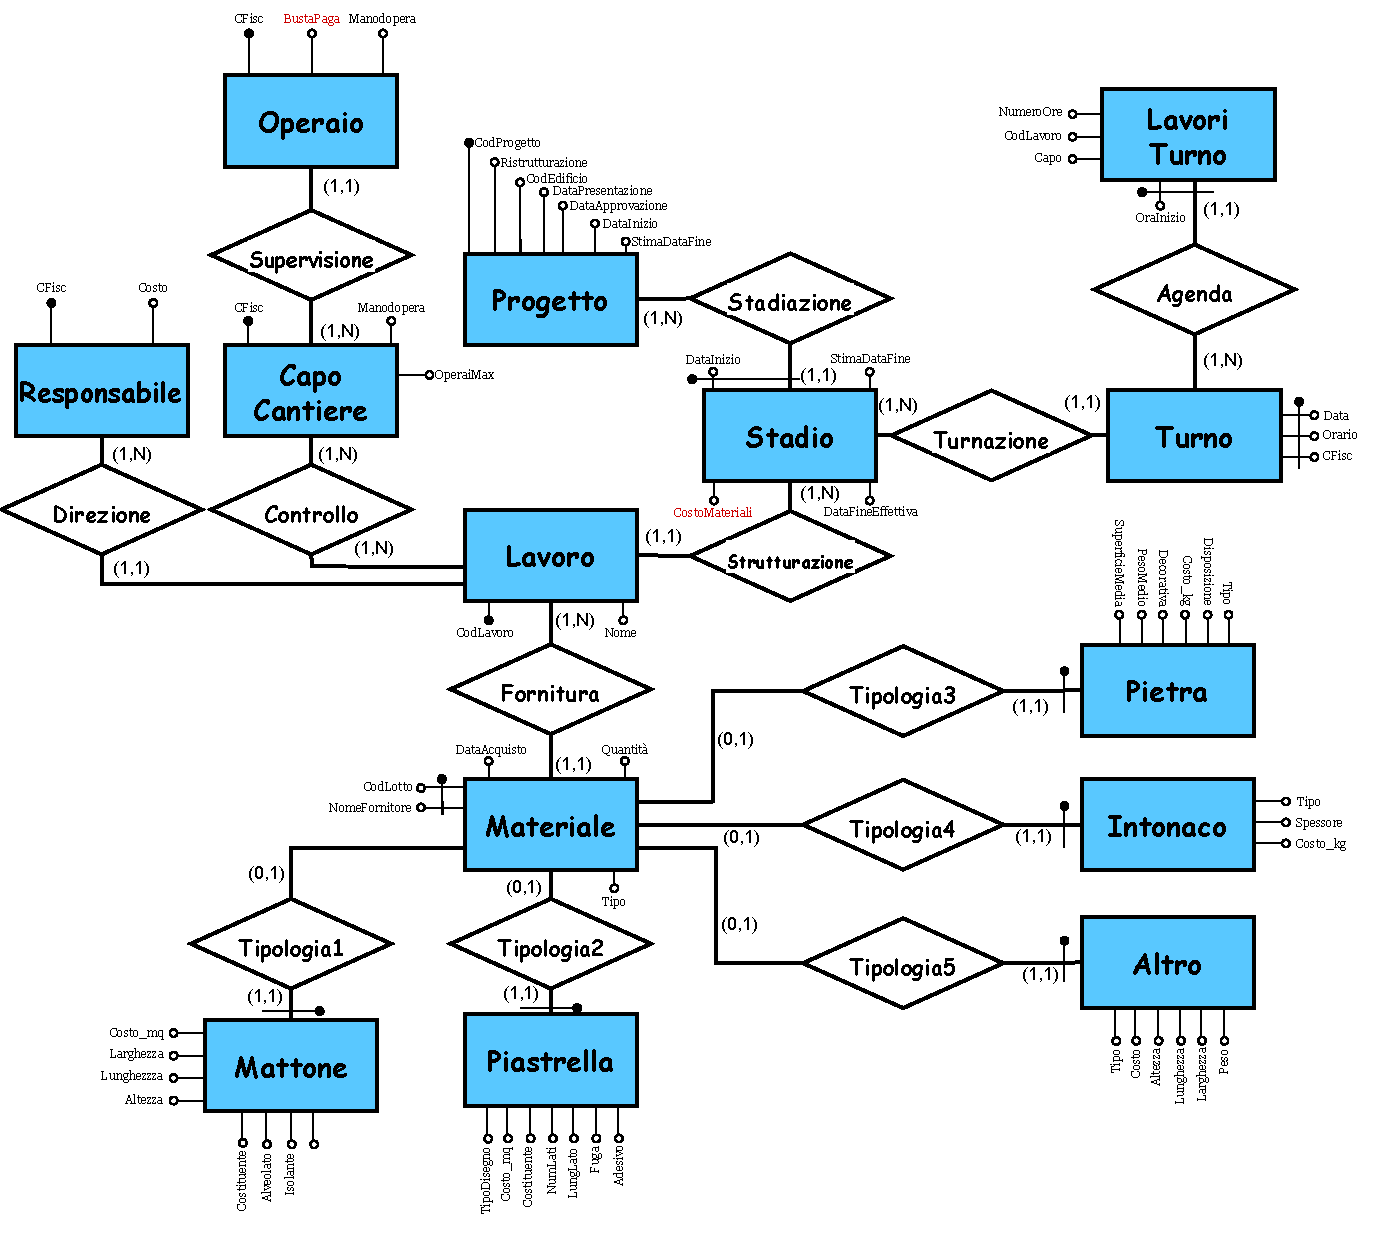
\includegraphics[scale=0.8]{sezione_operazione5.pdf}
            \end{center}
            
            \subsection{Tavola dei Volumi Interessati}
            \begin{tabular}{|p{4cm}|p{1cm}|p{3cm}|p{8cm}|}
                \hline
                \textbf{Concetto} & \textbf{Tipo} & \textbf{Volume} & \textbf{Considerazioni} \\ \hline
                Stadio & E & 14*3 = 42 & Ipotizzando 3 Stadi per ogni Progetto \\ \hline
                Strutturazione & R & 1.620 & Stesso volume di Lavoro \\ \hline
                Fornitura & R & 3.240 & Stesso volume di Materiale \\ \hline
                Materiale & E & 3*1.080 = 3.240 & Ipotizzando che una Parte sia composta mediamente da 3 materiali \\ \hline
                Mattone & E & 0,2*1.080 = 216 & Ipotizzando che il 20\% dei Materiali siano Mattone \\ \hline
                Piastrella & E & 0,2*1.080 = 216 & Ipotizzando che il 20\% dei Materiali siano Piastrella \\ \hline
                Pietra & E & 0,2*1.080 = 216 & Ipotizzando che il 20\% dei Materiali siano Pietra \\ \hline
                Intonaco & E & 0,3*1.080 =  324 & Ipotizzando che il 30\% dei Materiali siano Intonaco \\ \hline
                Altro & E & 0,1*1.080 = 108 & Ipotizzando che il 10\% dei Materiali siano Altro \\ \hline
            \end{tabular}
            
            \subsection{Tavola degli Accessi}
            \begin{tabular}{|c|c|c|c|p{4cm}|p{3cm}|c|}
                \hline
                \textbf{id} & \textbf{Concetto} & \textbf{Costrutto} & \textbf{Tipo} & \textbf{Considerazioni} & \textbf{Accessi} & \textbf{Dim(Ris)} \\ \hline
                1 & Strutturazione & R & Lettura & Leggo i lavori relativi allo stadio & Vol(Strutturaz.) = 1.620 & 39 \\ \hline
                2 & Fornitura & R & Lettura & Leggo tutte le forniture di tutti i lavori dello stadio & Vol(Fornitura) *39 = 3.240*39 = 126.360 & ~ \\ \hline
                3 & Materiale & E & Lettura & Leggo la quantità di tutte le forniture & 2*39 = 78 & ~ \\ \hline
                4 & Materiale\_i & E & Lettura & Leggo il costo di ogni Fornitura & 2*39 = 78 & ~ \\ \hline
                \multicolumn{5}{|c|}{Totale degli accessi per 1 volta annuale} & \multicolumn{2}{|c|}{128.136} \\ \hline
                \multicolumn{5}{|c|}{Totale degli accessi per 540 volte mensili} & \multicolumn{2}{|c|}{128.136*18 = 2.306.448} \\ \hline
            \end{tabular}

            \subsection{Valutazione della Ridondanza Costo in Stadio}
                Dato l'elevato numero di accessi necessari per portare a termine l'operazione, anche in questo caso si decide di valutare l'inserimento di una ridondanza che possa diminuirne gli accessi. In particolare si è deciso di valutare la ridondanza CostoMateriali come attributo dell'entità Stadio. In questo modo, al termine di ogni inserimento in Pietra, Mattone, Piastrella, Intonaco o Altro, si aggiorna la ridondanza per poi effettuare meno accessi nel momento della chiamata all'operazione.

                Come detto in precedenza, la Tavola dei Volumi si riferisce a 5 anni di attività della Base di Dati, occorre quindi stimare il numero dei nuovi inserimenti nelle entità sopra citate ogni anno. Questa stima può essere fatta dividendo la somma dei Volumi di Pietra, Mattone, Piastrella, Intonaco e Altro presenti nella Base di Dati per 5, ottenedo quindi 648 nuovi materiali all'anno.

            \subsubsection{Tavola degli Accessi con Ridondanza}
            \begin{tabular}{|c|c|c|c|p{4cm}|p{3cm}|c|}
                \hline
                \textbf{id} & \textbf{Concetto} & \textbf{Costrutto} & \textbf{Tipo} & \textbf{Considerazioni} & \textbf{Accessi} & \textbf{Dim(Ris)} \\ \hline
                1 & Stadio & E & Lettura & Leggo l'attributo ridondante & 18 & ~ \\ \hline
                2 & Materiale & E & Lettura & Leggo la quantità dei materiali acquistati & 648 & ~ \\ \hline
                3 & Fornitura & R & Lettura & Leggo i lavori nei quali ho utilizzato i materiali &  648 & ~ \\ \hline
                4 & Strutturazione & R & Lettura & Leggo gli stadi a cui appartengono i lavori & 648 & ~ \\ \hline
                5 & Stadio & E & Lettura & Leggo attributo ridondante & 648 & ~ \\ \hline
                6 & Stadio & E & Scrittura & Scrivo valore aggiornato & 2*648 & ~ \\ \hline
                \multicolumn{5}{|c|}{Totale degli accessi annuali} & \multicolumn{2}{|c|}{3.906} \\ \hline
            \end{tabular}

        \newpage

        \section{Operazione 6 - nuovoOperaio}
            L'operazione ha lo scopo di inserire un Operaio all'interno della Base di Dati. L'operaio in questione dovrà rispecchiare un criterio fondamentale per il mantenimento della logica dell'applicativo, ovvero il fare capo ad un Capo Cantiere il cui numero di Operai supervisionati non superi il numero massimo di individui che quel particolare Capo Cantiere può supervisionare.

            Considerata la Tavola dei Volumi relativa a 5 anni di utilizzo del database, possiamo stimare un numero di chiamate pari al rapporto tra il volume della tabella Operaio e il numero di anni presi in considerazione dalla Tavola dei Volumi.
        
        \begin{center}
            \begin{tabular}{|c|c|c|}
                \hline
                \rowcolor{viola} \textbf{Input} & \textbf{Output} & \textbf{Frequenza} \\ \hline
                Attributi di Operaio & Nessuno & Vol(Operaio) / 5 = 108 all'anno \\ \hline
            \end{tabular}
        \end{center}
        
        \subsection{Sezione di Diagramma Interessato}
        \begin{center}
            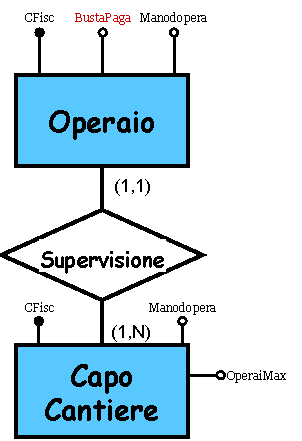
\includegraphics[scale=1.2]{sezione_operazione6.pdf}
        \end{center}
        
        \subsection{Tavola dei Volumi Interessati}
        \begin{tabular}{|p{4cm}|p{1cm}|p{3cm}|p{8cm}|}
            \hline
            \textbf{Concetto} & \textbf{Tipo} & \textbf{Volume} & \textbf{Considerazioni} \\ \hline
            Capo Cantiere & E & 45 & Ipotizzato \\ \hline
            Supervisione & R & 540 & Stesso volume di Operaio \\ \hline
            Operaio & E & 12*45 = 540 & Ipotizzando in media 12 Operai per Capo Cantiere \\ \hline
        \end{tabular}
        
        \subsection{Tavola degli Accessi}
        \begin{tabular}{|c|c|c|c|p{4cm}|p{3cm}|c|}
            \hline
            \textbf{id} & \textbf{Concetto} & \textbf{Costrutto} & \textbf{Tipo} & \textbf{Considerazioni} & \textbf{Accessi} & \textbf{Dim(Ris)} \\ \hline
            1 & CapoCantiere & E & Lettura & Leggo OperaiMax & 1 & ~ \\ \hline
            2 & Supervisione & R & Lettura & Conto le righe degli operai di quel capo & Vol(Super.)*1 = 540 & ~ \\ \hline
            3 & Operaio & E & Scrittura & Inserisco la tupla & 1 & ~ \\ \hline
            \multicolumn{5}{|c|}{Totale degli accessi per 1 volta} & \multicolumn{2}{|c|}{543} \\ \hline
            \multicolumn{5}{|c|}{Totale degli accessi per 540 volte} & \multicolumn{2}{|c|}{540*108 = 58.320} \\ \hline
        \end{tabular}

        \section{Operazione 7 - valutaAlert}
            Dato un Alert, la funzione si occupa di trovare tutte le informazioni necessarie per sapere quale Parte l'ha generato. Una operazione del genere è fondamentale per garantire la sicurezza degli Edifici, in quanto in base alla tipologia di Alert potrebbero essere necessarie delle azioni di manutenzione straordinaria urgenti.

            Una stima della pericolosità dell'Alert può essere data considerando il valore Soglia presente nel Sensore che ha generato quel particolare Alert e confrontandolo con il valore misurato nell'Alert.

        \begin{center}
            \begin{tabular}{|c|c|c|}
                \hline
                \rowcolor{viola} \textbf{Input} & \textbf{Output} & \textbf{Frequenza} \\ \hline
                Alert & CodEdificio, Piano, IDVano, NomeParte, Pericolosità (Float) & 10 volte ogni 2 mesi \\ \hline
            \end{tabular}
        \end{center}

        \subsection{Sezione di Diagramma Interessato}
        \begin{center}
            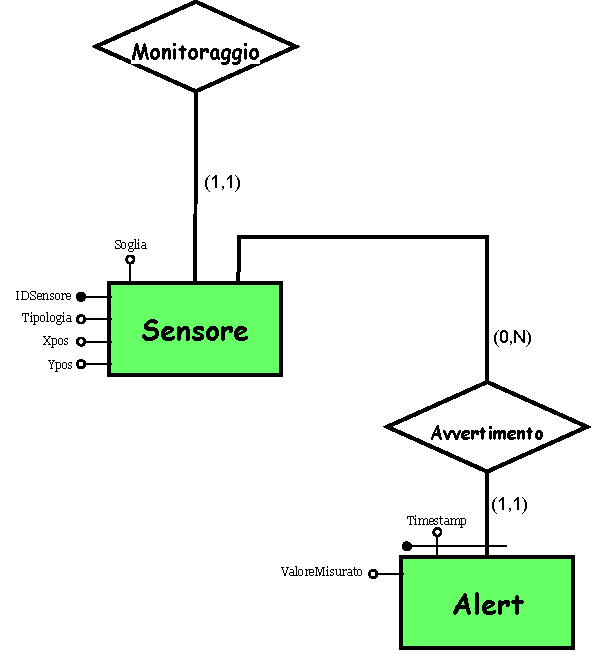
\includegraphics{sezione_operazione7.pdf}
        \end{center}

        \subsection{Tavola dei Volumi Interessati}
        \begin{tabular}{|p{4cm}|p{1cm}|p{3cm}|p{8cm}|}
            \hline
            \textbf{Concetto} & \textbf{Tipo} & \textbf{Volume} & \textbf{Considerazioni} \\ \hline
            Alert & E & 0,3*1.131.500 = 339.450 & Ipotizzando chen il 30\% delle Misurazioni generino un Alert \\ \hline
            Sensore & E & 310 & Ipotizzato \\ \hline
            Monitoraggio & R & 310 & Stesso volume di Sensore \\ \hline
        \end{tabular}

        \subsection{Tavola degli Accessi}
        \begin{tabular}{|c|c|c|c|p{4cm}|p{3cm}|p{3cm}|}
            \hline
            \textbf{id} & \textbf{Concetto} & \textbf{Costrutto} & \textbf{Tipo} & \textbf{Considerazioni} & \textbf{Accessi} & \textbf{Dim(Ris)} \\ \hline
            1 & Alert & E & Lettura & Leggo ValoreMisurato & 1 & ~ \\ \hline
            2 & Sensore & E & Lettura & Leggo Soglia & 1 & ~ \\ \hline
            3 & Monitoraggio & R & Lettura & Leggo codEdificio, IDVano, Nome, Piano & 1 & ~ \\ \hline
            \multicolumn{5}{|c|}{Totale degli accessi per 1 volta} & \multicolumn{2}{|c|}{3} \\ \hline
            \multicolumn{5}{|c|}{Totale degli accessi per 10 volte} & \multicolumn{2}{|c|}{3*10 = 30} \\ \hline
        \end{tabular}

        \section{Operazione 8 - materialiLavoro}
        Dato un Lavoro, l'operazione materialiLavoro si prefissa l'obiettivo di trovare, all'interno del Lavoro identificato dal codice dato in input, i Materiali necessari per portarlo a termine.

        È sensato pensare di eseguire questa operazione, per valutare i Materiali utilizzati per portarlo alla conclusione, una volta per ogni Lavoro concluso. Dunque, si calcola la frequenza come il volume della tabella Lavoro diviso per il numero di anni a cui fa riferimento la Tabella dei Volumi, considerando così una frequenza annua di 324 volte. 
        \begin{center}
            \begin{tabular}{|c|c|c|}
                \hline
                \rowcolor{viola} \textbf{Input} & \textbf{Output} & \textbf{Frequenza} \\ \hline
                CodLavoro & Costo (Float) & 324 volte all'anno \\ \hline
            \end{tabular}
        \end{center}

        \subsection{Sezione di Diagramma Interessato}
        \begin{center}
            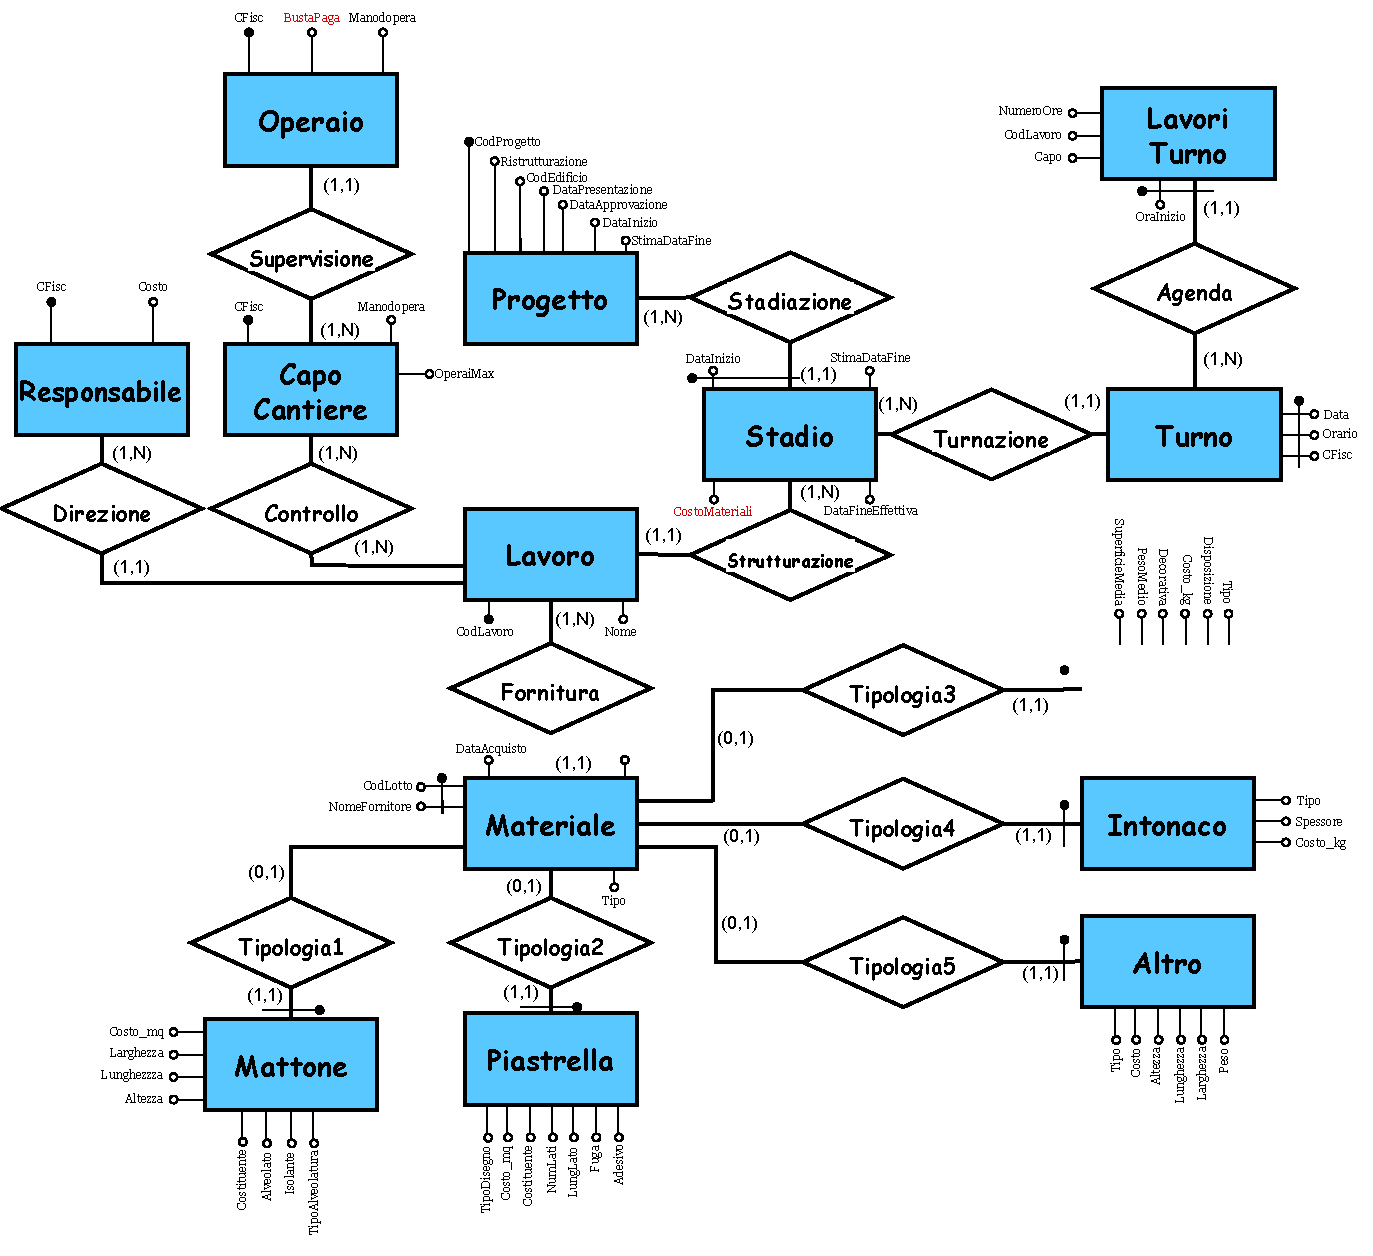
\includegraphics[scale=0.9]{sezione_operazione8.pdf}
        \end{center}

        \subsection{Tavola dei Volumi Interessati}
        \begin{tabular}{|p{4cm}|p{1cm}|p{3cm}|p{8cm}|}
            \hline
            \textbf{Concetto} & \textbf{Tipo} & \textbf{Volume} & \textbf{Considerazioni} \\ \hline
            Lavoro & E & 0,5*3.240 = 1.620 & Ipotizzando 2 Materiali per ogni Lavoro \\ \hline
            Fornitura & R & 3.240 & Stesso volume di Materiale \\ \hline
            Materiale & E & 3*1.080 = 3.240 & Ipotizzando che una Parte sia composta mediamente da 3 materiali \\ \hline
            Mattone & E & 0,2*1.080 = 216 & Ipotizzando che il 20\% dei Materiali siano Mattone \\ \hline
            Piastrella & E & 0,2*1.080 = 216 & Ipotizzando che il 20\% dei Materiali siano Piastrella \\ \hline
            Pietra & E & 0,2*1.080 = 216 & Ipotizzando che il 20\% dei Materiali siano Pietra \\ \hline
            Intonaco & E & 0,3*1.080 =  324 & Ipotizzando che il 30\% dei Materiali siano Intonaco \\ \hline
            Altro & E & 0,1*1.080 = 108 & Ipotizzando che il 10\% dei Materiali siano Altro \\ \hline
        \end{tabular}
    
        \subsection{Tavola degli Accessi}
        \begin{tabular}{|c|c|c|c|p{4cm}|p{3cm}|p{3cm}|}
            \hline
            \textbf{id} & \textbf{Concetto} & \textbf{Costrutto} & \textbf{Tipo} & \textbf{Considerazioni} & \textbf{Accessi} & \textbf{Dim(Ris)} \\ \hline
            1 & Fornitura & R & Lettura & Leggo i Materiali relativi al Lavoro & Vol(Fornitura) = 3.240 & 2 \\ \hline
            2 & Materiale & E & Lettura & Leggo Quantita & 2 & ~ \\ \hline
            3 & Materiale\_i & E & Lettura & Leggo le informazioni del Materiale & 2 & ~ \\ \hline
            \multicolumn{5}{|c|}{Totale degli accessi per 1 volta} & \multicolumn{2}{|c|}{3.244} \\ \hline
            \multicolumn{5}{|c|}{Totale degli accessi per 324 volte} & \multicolumn{2}{|c|}{3.244*324 = 1.051.056} \\ \hline
        \end{tabular}

\part{Modello Logico}

    \chapter{Descrizione Schema Logico}
    Per semplicità notazionale, viene riportato il tipo degli attributi subito sopra al nome dell'attributo stesso.

    In questa notazione: $vc(i)$ rappresenta il tipo VARCHAR(i), $c(i)$ rappresenta il tipo CHAR(i), $ts$ rappresenta il tipo TIMESTAMP, e $int$ e $float$ rappresentano rispettivamente i tipi INT e FLOAT.

    \vspace{0.5cm}
    \begin{flushleft}
        \begin{footnotesize}
            Calamita(\underline{$\overset{vc(100)}{AreaGeografica}$, $\overset{date}{Data}$ , $\overset{vc(100)}{Tipo}$}, $\overset{float}{LongEpicentro}$, $\overset{float}{LatEpicentro}$)
            \vspace{0.5cm}
    
            Rischio(\underline{$\overset{vc(100)}{AreaGeografica}$}, $\overset{float}{Tipo}$, $\overset{date}{Data}$, $\overset{int}{Coefficiente}$)
            \vspace{0.5cm}
            
            AreaGeografica(\underline{$\overset{vc(100)}{Nome}$})
            \vspace{0.5cm}
            
            Eventualita(\underline{$\overset{c(5)}{Edificio}$, $\overset{vc(100)}{AreaGeografica}$, $\overset{date}{Data}$, $\overset{vc(100)}{TipoCalamita}$}, $\overset{int}{Gravita}$)
            \vspace{0.5cm}
            
            Edificio(\underline{$\overset{c(5)}{CodEdificio}$}, $\overset{tinyint}{Esistente}$, $\overset{vc(100)}{AreaGeografica}$, $\overset{float}{Longitudine}$, $\overset{float}{Latitudine}$)
            \vspace{0.5cm}
            
            Funzione(\underline{$\overset{vc(100)}{NomeFunz}$}, $\overset{c(5)}{IDVano}$, $\overset{int}{Piano}$, $\overset{c(5)}{Edificio}$)
            \vspace{0.5cm}
            
            Pianta(\underline{$\overset{int}{Piano}$, $\overset{c(5)}{Edificio}$}, $\overset{int}{NLati}$)
            \vspace{0.5cm}
            
            Vano(\underline{$\overset{c(5)}{IDVano}$, $\overset{int}{Piano}$, $\overset{c(5)}{Edificio}$}, $\overset{float}{LungMax}$, $\overset{float}{HMax}$, $\overset{float}{LargMax}$, $\overset{float}{HMin}$)
            \vspace{0.5cm}
            
            AccessoI(\underline{$\overset{c(5)}{IDPuntoAccesso}$, $\overset{c(5)}{IDVano}$, $\overset{int}{Piano}$, $\overset{c(5)}{Edificio}$}, $\overset{vc(5)}{Orientamento}$)
            \vspace{0.5cm}
            
            PuntoAccessoInterno(\underline{$\overset{c(5)}{IDPuntoAccesso}$}, $\overset{vc(45)}{Tipo}$, $\overset{float}{Larghezza}$, $\overset{float}{Altezza}$)
            \vspace{0.5cm}
            
            PuntoAccessoEsterno(\underline{$\overset{c(5)}{IDPuntoAccesso}$}, $\overset{float}{Larghezza}$, $\overset{float}{Altezza}$, $\overset{vc(6)}{Orientamento}$, $\overset{vc(45)}{Tipo}$, $\overset{c(5)}{IDVano}$, $\overset{int}{Piano}$, $\overset{c(5)}{Edificio}$)
            \vspace{0.5cm}
            
            Finestra(\underline{$\overset{c(5)}{IDFinestra}$}, $\overset{c(5)}{IDVano}$, $\overset{int}{Piano}$, $\overset{c(5)}{Edificio}$, $\overset{float}{Larghezza}$, $\overset{float}{Altezza}$, $\overset{vc(6)}{Orientamento}$)        \vspace{0.5cm}
            
            Parte(\underline{$\overset{c(5)}{Nome}$, $\overset{c(5)}{Vano}$, $\overset{int}{Piano}$, $\overset{c(5)}{Edificio}$}, $\overset{float}{Superficie}$, $\overset{tinyint}{Ext}$)
            \vspace{0.5cm}
            
            Sensore(\underline{$\overset{c(5)}{IDSensore}$}, $\overset{vc(100)}{Tipologia}$, $\overset{float}{XPos}$, $\overset{float}{YPos}$, $\overset{float}{ZPos}$, $\overset{float}{Soglia}$, $\overset{c(5)}{NomeParte}$, $\overset{c(5)}{Vano}$, $\overset{int}{Piano}$, $\overset{c(5)}{Edificio}$)
            \vspace{0.5cm}
            
            Alert(\underline{$\overset{ts}{Timestamp}$, $\overset{c(5)}{IDSensore}$}, $\overset{float}{ValoreMisurato}$)
            \vspace{0.5cm}
            
            Posizione(\underline{$\overset{ts}{Timestamp}$, $\overset{c(5)}{IDSensore}$}, $\overset{float}{Larghezza}$)
            \vspace{0.5cm}
            
            Temperatura(\underline{$\overset{ts}{Timestamp}$, $\overset{c(5)}{IDSensore}$}, $\overset{float}{TemperaturaRilevata}$)
            \vspace{0.5cm}
            
            Pluviometro(\underline{$\overset{ts}{Timestamp}$, $\overset{c(5)}{IDSensore}$}, $\overset{float}{Precipitazione}$)
            \vspace{0.5cm}
            
            Giroscopio(\underline{$\overset{ts}{Timestamp}$, $\overset{c(5)}{IDSensore}$}, $\overset{float}{Wx}$, $\overset{float}{Wy}$, $\overset{float}{Wz}$)
            \vspace{0.5cm}
            
            Accelerometro(\underline{$\overset{ts}{Timestamp}$, $\overset{c(5)}{IDSensore}$}, $\overset{float}{X}$, $\overset{float}{Y}$, $\overset{float}{Z}$)
            \vspace{0.5cm}
            
            Materiale(\underline{$\overset{c(5)}{CodLotto}$, $\overset{vc(100)}{NomeFornitore}$}, $\overset{vc(100)}{Tipo}$, $\overset{int}{Quantita}$, $\overset{date}{DataAcquisto}$, $\overset{c(5)}{CodLavoro}$, $\overset{c(5)}{NomeParte}$, $\overset{c(5)}{Vano}$, $\overset{int}{Piano}$, $\overset{c(5)}{Edificio}$)
            \vspace{0.5cm}
            
            Pietra(\underline{$\overset{c(5)}{CodLotto}$, $\overset{vc(100)}{NomeFornitore}$}, $\overset{float}{SuperficieMedia}$, $\overset{float}{PesoMedio}$, $\overset{tinyint}{Decorativa}$, $\overset{float}{Costo_kg}$, $\overset{vc(11)}{Disposizione}$, $\overset{vc(100)}{Tipo}$)
            \vspace{0.5cm}
            
            Mattone(\underline{$\overset{c(5)}{CodLotto}$, $\overset{vc(100)}{NomeFornitore}$},$\overset{float}{Costo_mq}$, $\overset{float}{Larghezza}$, $\overset{float}{Lunghezza}$, $\overset{float}{Altezza}$, $\overset{vc(100)}{Costituente}$, $\overset{tinyint}{Alveolato}$, $\overset{tinyint}{Isolante}$, $\overset{vc(100)}{TipoAlveolatura}$)
            \vspace{0.5cm}
            
            Piastrella(\underline{$\overset{c(5)}{CodLotto}$, $\overset{vc(100)}{NomeFornitore}$},$\overset{vc(100)}{TipoDisegno}$, $\overset{float}{Costo_mq}$, $\overset{vc(100)}{Costituente}$, $\overset{int}{NumLati}$, $\overset{float}{LungLato}$, $\overset{float}{Fuga}$, $\overset{vc(100)}{Adesivo}$)
            \vspace{0.5cm}
            
            Intonaco(\underline{$\overset{c(5)}{CodLotto}$, $\overset{vc(100)}{NomeFornitore}$},$\overset{vc(100)}{Tipo}$, $\overset{float}{Spessore}$, $\overset{float}{Costo_kg}$)
            \vspace{0.5cm}
            
            Altro(\underline{$\overset{c(5)}{CodLotto}$, $\overset{vc(100)}{NomeFornitore}$}, $\overset{vc(100)}{Tipo}$, $\overset{float}{Costo}$, $\overset{float}{Altezza}$, $\overset{float}{Lunghezza}$, $\overset{float}{Larghezza}$, $\overset{float}{Peso}$)
            \vspace{0.5cm}
            
            Lavoro(\underline{$\overset{c(5)}{CodLavoro}$}, $\overset{vc(100)}{Nome}$, $\overset{c(5)}{Responsabile}$, $\overset{date}{DataInizioStadio}$, $\overset{c(5)}{CodProgetto}$)
            \vspace{0.5cm}
            
            Responsabile(\underline{$\overset{c(5)}{CFisc}$}, $\overset{float}{Costo}$)        
            \vspace{0.5cm}
            
            Controllo(\underline{$\overset{c(5)}{CodLavoro}$, $\overset{c(16)}{CapoCantiere}$})        
            \vspace{0.5cm}
            
            CapoCantiere(\underline{$\overset{c(16)}{CFisc}$}, $\overset{float}{Manodopera}$, $\overset{int}{OperaiMax}$)        
            \vspace{0.5cm}
            
            Operaio(\underline{$\overset{c(16)}{CFisc}$}, $\overset{float}{Manodopera}$, $\overset{c(16)}{CapoCantiere}$, $\overset{float}{BustaPaga}$)     
            \vspace{0.5cm}
            
            Stadio(\underline{$\overset{date}{DataInizio}$, $\overset{c(5)}{CodProgetto}$}, $\overset{date}{StimaDataFine}$, $\overset{date}{DataFineEffettiva}$, $\overset{float}{Costo}$)        
            \vspace{0.5cm}
            
            Progetto(\underline{$\overset{c(5)}{CodProgetto}$}, $\overset{tinyint}{Ristrutturazione}$, $\overset{date}{DataPresentazione}$, $\overset{date}{DataApprovazione}$, $\overset{date}{DataInizio}$, $\overset{date}{StimaDataFine}$, $\overset{c(5)}{CodEdificio}$)        
            \vspace{0.5cm}
            
            Turno(\underline{$\overset{date}{Data}$, $\overset{c(16)}{CFisc}$, $\overset{vc(100)}{Orario}$}, $\overset{date}{DataInizioStadio}$, $\overset{c(5)}{CodProgetto}$)        
            \vspace{0.5cm}
            
            LavoriTurno(\underline{$\overset{int}{OraInizio}$, $\overset{date}{Data}$, $\overset{c(5)}{CFiscLavoratore}$, $\overset{vc(10)}{Orario}$}, $\overset{int}{NumeroOre}$, $\overset{c(5)}{CodLavoro}$, $\overset{c(16)}{Capo}$)        
            \vspace{0.5cm}
        \end{footnotesize}        
    \end{flushleft}

    \chapter{Analisi delle Dipendenze Funzionali e Normalizzazione}
        
        Per tutte le tabelle descritte sopra, ad eccezione di Edificio, Sensore e Stadio, la chiave è unica e non ci sono dipendenze funzionali non banali. Esse sono quindi in BCNF.
        
        \section{Tabella Edificio}
        
        Nella tabella Edificio sono presenti le seguenti dipendenze funzionali:

        \begin{itemize}
            \item \emph{CodEdificio} $\rightarrow$ \emph{Intera Tupla} \\ Banale poichè ho la chiave primaria a sinistra.
            
            \item \emph{Latitudine}, \emph{Longitudine} $\rightarrow$ \emph{Intera Tupla} \\ L’implicante costituisce un’altra chiave di Edificio, dato che in un determinato punto della Terra descritto dalle due coordinate posso costruire un solo edificio.
        \end{itemize}

        Quindi, visto che per tutte le dipendenze non banali l'implicante è una chiave, Edificio è in BCNF.

        \section{Tabella Sensore}
        
        Nella tabella Sensore sono presenti le seguenti dipendenze funzionali:

        \begin{itemize}
            \item \emph{IDSensore} $\rightarrow$ \emph{Intera Tupla} \\ Banale poiché ho la chiave primaria a sinistra
            
            \item \emph{Parte}, \emph{Piano}, \emph{Vano}, \emph{Edificio}, \emph{XPos}, \emph{YPos} $\rightarrow$ \emph{Intera Tupla} \\ L’implicante costituisce un’altra chiave di Sensore, dato che in un determinato punto $(XPos, YPos)$ di una parte di un edificio, può essere posizionato un solo sensore. 
        \end{itemize}

        Quindi, visto che per tutte le dipendenze non banali l’implicante è una chiave, Sensore è in BCNF.

        \section{Tabella Stadio}
        
        Nella tabella Stadio sono presenti le seguenti dipendenze funzionali:

        \begin{itemize}
            \item \emph{CodProgetto}, \emph{DataInizio} $\rightarrow$ \emph{Intera Tupla} \\ Banale poichè ho la chiave primaria a sinistra.
            
            \item \emph{CodProgetto}, \emph{StimaDataFine} $\rightarrow$ \emph{Intera Tupla} \\ L'implicante costituisce un'altra chiave di Stadio, dato che, vista la sequenzialità degli stadi dei progetti, preso un Progetto, per una \emph{}StimaDataFine potrò avere un solo Stadio corrispondente.
        \end{itemize}

        Quindi, visto che per tutte le dipendenze non banali l’implicante è una chiave, Stadio è in BCNF.

    \chapter{Vincoli di Integrità}
        \section{Vincoli di Integrità Referenziale}
            Sono presenti tutti i vincoli di integrità referenziale generati dalla traduzione dello schema ER. 
            
            Inoltre, sono stati implementati i seguenti vincoli:
            \begin{itemize}
                \item L'attributo Capo in LavoriTurno non può contenere valori non presenti in CFisc di Capo
                \item L'attributo CodEdificio in Progetto non può contenere valori non presenti in CodEdidifio di Edificio
                \item L'attributo CFisc in Turno non può contenere valori non presenti in CFisc di CapoCantiere e Operaio
            \end{itemize}
        \section{Vincoli di Integrità Generici}
            \begin{itemize}
                \item Un Operaio non può avere un Capo diverso dal suo
                \item Un Punto d'Accesso Interno collega 2 vani
                \item L'Edificio in Materiale deve corrispondere all'Edificio del Lavoro
                \item Un lavoratore non può svolgere contemporaneamente più lavori
            \end{itemize}
        \section{Vincoli di Tupla}
            \begin{itemize}
                \item L'attributo Tipo in Calamita deve essere una stringa ``Sismico" o ``Idrogeologico"
                \item L'attributo Gravita in Eventualita deve essere un intero compreso fra 0 e 100
                \item L'attributo Orientamento in Finestra deve essere una stringa fra le seguenti:
                
                ``Nord",``Sud",``Est",``Ovest",``NordEst",``NordOvest",``SudEst",``SudOvest"
                \item L'attributo Orientamento in PA\_Esterno deve essere una stringa fra le seguenti: 
                
                ``Nord",``Sud",``Est",``Ovest",``NordEst",``NordOvest",``SudEst",``SudOvest"
                \item L'attributo Tipologia in Sensore deve essere una stringa fra le seguenti: 
                
                ``Giroscopio",``Temperatura",``Posizione",``Pluviometro",``Accelerometro"
                \item L'attributo Tipo in Materiale deve essere una stringa fra le seguenti: 
                
                ``Pietra",``Intonaco",``Altro",``Piastrella",``Mattone"
                \item L'attributo Orario in Turno deve essere una stringa fra le seguenti: ``Mattutino",``Pomeridiano"
                \item L'attributo OraInizio in LavoriTurno deve essere compreso tra 7 e 18
                \item Le Date in Progetto devono essere coerenti temporalmente
                \item In Edificio, l'attributo Latitudine è compreso fra -90 e 90, e l'attributo Longitudine tra -180 e 180
                \item In Calamita, l'attributo LatEpicentro è compreso fra -90 e 90, e l'attributo LongEpicentro tra -180 e 180
            \end{itemize}

            \chapter{Implementazione funzioni Analytics}
                \section{consigliIntervento}
                I consigli di intervento assegnati quando si chiama consigliIntervento dipendono dai rischi nella seguente logica.

                Consideriamo gli ultimi alert generati dai sensori dellàedificio in questione. Questi alert avranno sicuramente un valore anomalo, altrimenti non sarebbero stati generati, e quindi presentano un piccolo contributo che fa peggiorare logicamente l'intera valutazione dei consigli.

                Di ogni alert così trovato, posso rendermi conto di quanto grava sulla valutazione dell'intervento constatando quanto si è scostato in percentuale dalla soglia.

                Una volta assegnato lo scostamento percentuale ad ogni alert, questo valore verrà ulteriormente incrementato, e quindi aggravato, da un contributo dato dal valore stesso moltiplicato per l'attuale coefficiente di rischio presente nell'area geografica in cui è situato l'edificio.

                Considerato quindi questo ultimo dato, viene fatta una stima dipendente anche dal numero di piani che l'edificio presenta, e dal piano in cui il sensore che ha generato quell'alert è posizionato.

                In questi termini viene fatta una valutazione composta dal genere di intervento che si deve fare e dal numero di giorni entro il quale dovrebbe essere effettuato l'intervento.

                Per quanto riguarda il genere di intervento, ovviamente dipende da quale tipo di sensore stiamo considerando. Nel caso in cui un giroscopio oppure un accelerometro non sia situato all'ultimo piano dell'edificio, verrà consigliato un rifacimento di solaio al piano. D'altra parte, se proviene da un accelerometro oppure da un giroscopio, e però il sensore è posizionato all'ultimo piano, verrà consigliato un rifacimento della copertura. Nel caso in cui invece il sensore che ha generato quell'alert sia di posizione, occorre ovviamente risanare la parte, e questo in effetti viene consigliato.

                Invece per quanto riguarda i giorni consigliati entro il quale il problema dovrebbe essere risolto, vengono stimati tramite il valore calcolato in precedenza. Assumendo che sia un valore compreso fra 0 e 100, il range compreso tra 1 e 20 consiglierà un tempo di intervento di 60 giorni, e così via fino al tempo di intervento consigliato immediato.
                \section{stimaDanni}
                La stima dei danni viene assegnata tramite la definizione di \emph{stato} dell'edificio. Occorre quindi dare una definizione di tale oggetto.

                \begin{center}
                    $\displaystyle stato = \sum_{i=1}^{3} \Big[ \sum_{j=0}^{n} \Big( ( s_{s_{j}} - m_{s_{j}} ) \dfrac{1}{t_j} \Big) \Big] p_i$
                \end{center}
                con $s_{s_{j}}$ soglia del sensore j-esimo, $m_{s_{j}}$ misurazione del sensore j-esimo, $t_j$ distanza di mesi dalla chiamata della funzione alla misurazione del j-esimo valore, $p_i$ coefficiente che dipende dal tipo di sensore, $n$ numero di misurazioni dei sensori.

                La sommatoria interna si occupa di sommare ogni singolo scostamento delle misurazioni, in modo inversamente proporzionale al tempo, in mesi, in cui la misurazione è stata fatta. Questo perchè voglio dare maggiore peso alle misurazioni effettuate di recente, invece di quelle più lontane nel tempo. Inoltre, il valore così ottenuto viene moltiplicato per un coefficiente che dipende dal tipo di sensore che ha effettuato la misurazione. Questo perchè stiamo considerando la stima dei danni per un evento calamitoso sismico, e quindi i sensori piu influenti sono gli accelerometri e i giroscopi, invece dei sensori di posizione. Si e' deciso quindi di attribuire un valore di 0.2 ai sensori di posizione, e 0.4 ai giroscopi e agli accelerometri.

                La sommatoria più esterna invece si occupa di sommare tutti questi contributi, ottenendo quindi un valore sempre più grande quanto più le misurazioni sono vicine temporalmente e scostate dalla soglia.

                Una volta definito e calcolato lo stato di un edificio, occorre stimare i danni che un ipotetico evento sismico instaurerebbe nell'edificio stesso. Questo è possibile grazie alla gravità dell'ipotetico evento calamitoso. Innanzitutto dobbiamo osservare che lo stato di un edificio è un numero con la virgole, e positivo nel caso in cui i sensori si scostino molto dalla soglia. Osserviamo anche che la gravità di una calamità è un numero compreso fra 0 e 10.
                
                Si considerano infine le seguenti ipotesi: nel caso in cui lo stato sia positivo e la gravità bassa (ovvero compresa fra 0 e 5), l'edificio probabilmente non subirà danni. Altrimenti, se lo stato risulta sempre positivo ma la gravità è alta (ovvero compresa fra 5 e 10), significa che l'edificio si trova in buono stato ma anche che la gravità è considerevole, quindi verrà previsto un quantitativo di danni lievi. Altrimenti, se l'edificio ha uno stato negativo, e quindi non si trova in salute, e la gravità è bassa, comunque le condizioni dell'edificio non permetterebbero la sopportazione dell'evento sismico, e riporterebbe danni moderati. Infine, nel caso peggiore, ovvero il caso in cui lo stato sia negativo e la gravità alta, l'edificio potrebbe avere dei danni ingenti.
                
                
\end{document}